\documentclass[12pt,a4paper,openany]{book}
\usepackage{amssymb, amsmath}
% \usepackage[polish]{babel}
\usepackage[utf8]{inputenc}
\usepackage[T1]{fontenc}
\usepackage[dvips]{graphicx}
\setlength{\parindent}{7mm}
\setlength{\parskip}{4mm}
\usepackage{indentfirst}
\usepackage{mathtools}
\usepackage{enumitem}
\usepackage{titlesec}
\usepackage{paralist}
\usepackage{comment}
\usepackage{bigints}

\usepackage{accents}
\usepackage{amsthm}
\usepackage{graphicx}
\usepackage{amsmath}
\usepackage{float}
\restylefloat{table}

\usepackage{pdfpages}

\usepackage{xpatch}
\makeatletter
\xpatchcmd{\@thm}{\thm@headpunct{.}}{\thm@headpunct{}}{}{}
\makeatother

\graphicspath{ {figs/} }


\newcommand{\ubar}[1]{\underaccent{\bar}{#1}}
  \let\itemize\compactitem
  \let\enditemize\endcompactitem
  \let\enumerate\compactenum
  \let\endenumerate\endcompactenum
  \let\description\compactdesc
  \let\enddescription\endcompactdesc
  \pltopsep=1pt
  \plitemsep=1pt
  \plparsep=1pt

\newcommand\myeq{\mathrel{\overset{\makebox[0pt]{\mbox{\normalfont\tiny\sffamily $\lambda > 0$}}}{=}}}

\titleformat{\chapter}[display]   
{\normalfont\huge\bfseries}{\chaptertitlename\ \thechapter}{20pt}{\Huge}   
\titlespacing*{\chapter}{0pt}{-10pt}{40pt}

\titlespacing*{\section}{0pt}{1.\baselineskip}{\baselineskip}


\linespread{1.4}

\pagestyle{myheadings}
\pagestyle{plain}
\usepackage{geometry}
\newgeometry{tmargin=2.5cm, bmargin=2.5cm, lmargin=3cm, rmargin=2.5cm}
\newcommand\setItemnumber[1]{\setcounter{enumi}{\numexpr#1-1\relax}}
\newcommand*{\QEDB}{\hfill\ensuremath{\square}}
\newcommand{\ignore}[1]{}

\newcommand{\RomanNumeralCaps}[1]
    {\MakeUppercase{\romannumeral #1}}


\begin{document}

\begin{titlepage}
\begin{flushleft}
\end{flushleft}
\begin{center}
\textsc{{\huge Politechnika Warszawska}}
\end{center}
\bigskip
\bigskip
\begin{center}
\textsc{{\Large Wydział maszyn uczenia}}
\end{center}
\bigskip
\bigskip
\begin{center}
\begin{Large}
Kierunek: dip lerning
\end{Large}
\end{center}
\bigskip
\bigskip
\noindent\hrulefill
\begin{center}
\textsc{\textbf{{\large GANYYYY AYAAYAYAYA
\\}}}
\bigskip
\bigskip

{\large 
Adam Komorowski i Maciej Domagała}

\end{center}
\noindent\hrulefill
\bigskip
\bigskip
\begin{center}
\end{center}
\bigskip
\bigskip
\bigskip
\bigskip
\begin{center}
{\textsc{\large zdalnie, czerwiec 2021
}}
\end{center}
\end{titlepage}

\tableofcontents

\chapter*{Introduction}
\addcontentsline{toc}{chapter}{Introduction}

\chapter{Theory}

\section{Generative Adversarial Networks}

GENEZA

PODSTAWY ARCHITEKTURY - PRZYKŁAD

GENERATOR I DYSKRIMINATOR

STATE OF THE ARTS


\subsection{Metrics}

%https://www.coursera.org/lecture/build-better-generative-adversarial-networks-gans/inception-score-HxtYM - explained IS
%https://medium.com/octavian-ai/a-simple-explanation-of-the-inception-score-372dff6a8c7a - explained IS
%https://arxiv.org/pdf/1801.01973.pdf - IS paper
%https://machinelearningmastery.com/how-to-implement-the-inception-score-from-scratch-for-evaluating-generated-images/ - IS


%https://jonathan-hui.medium.com/gan-how-to-measure-gan-performance-64b988c47732 - all three metrics

\subsubsection*{Inception Score}
\subsubsection*{Fr\'echet Inception Distance}
\subsubsection*{Precision and Recall}

\section{CLIP model}

GENEZA

ZASTOSOWANIE

JAK ZROBIONE, PO CO


\section{Evolutionary Algorithms}

Evolutionary algorithms are a population-based heuristic methods of optimization. Algorithms from this family use computational implementations of processes related to natural selection, such as crossover, mutation and reproduction. Main idea of the algorithm is the \textit{survival of the fittest} principle inspired by Darwinian evolution theory, where main objective is to generate more and more \textit{fit} members of the population, while reducing the number of \textit{weak} units. That \textit{fitness} level is measured and described by \textit{fitness function}, which determines the quality of each population sample.\

In the following sections we will describe main algorithms of our interest that we will apply for latent search problem. 
\subsection{Genetic Algorithm}

% pics from: https://www.sciencedirect.com/science/article/pii/S1364815218305905

The Genetic Algorithm is one of the first methods used and defined as evolutionary algorithm. It is still used with success until today and the number of variations and different applications of the method still grows.

 \begin{figure}[ht!]
     \centering
     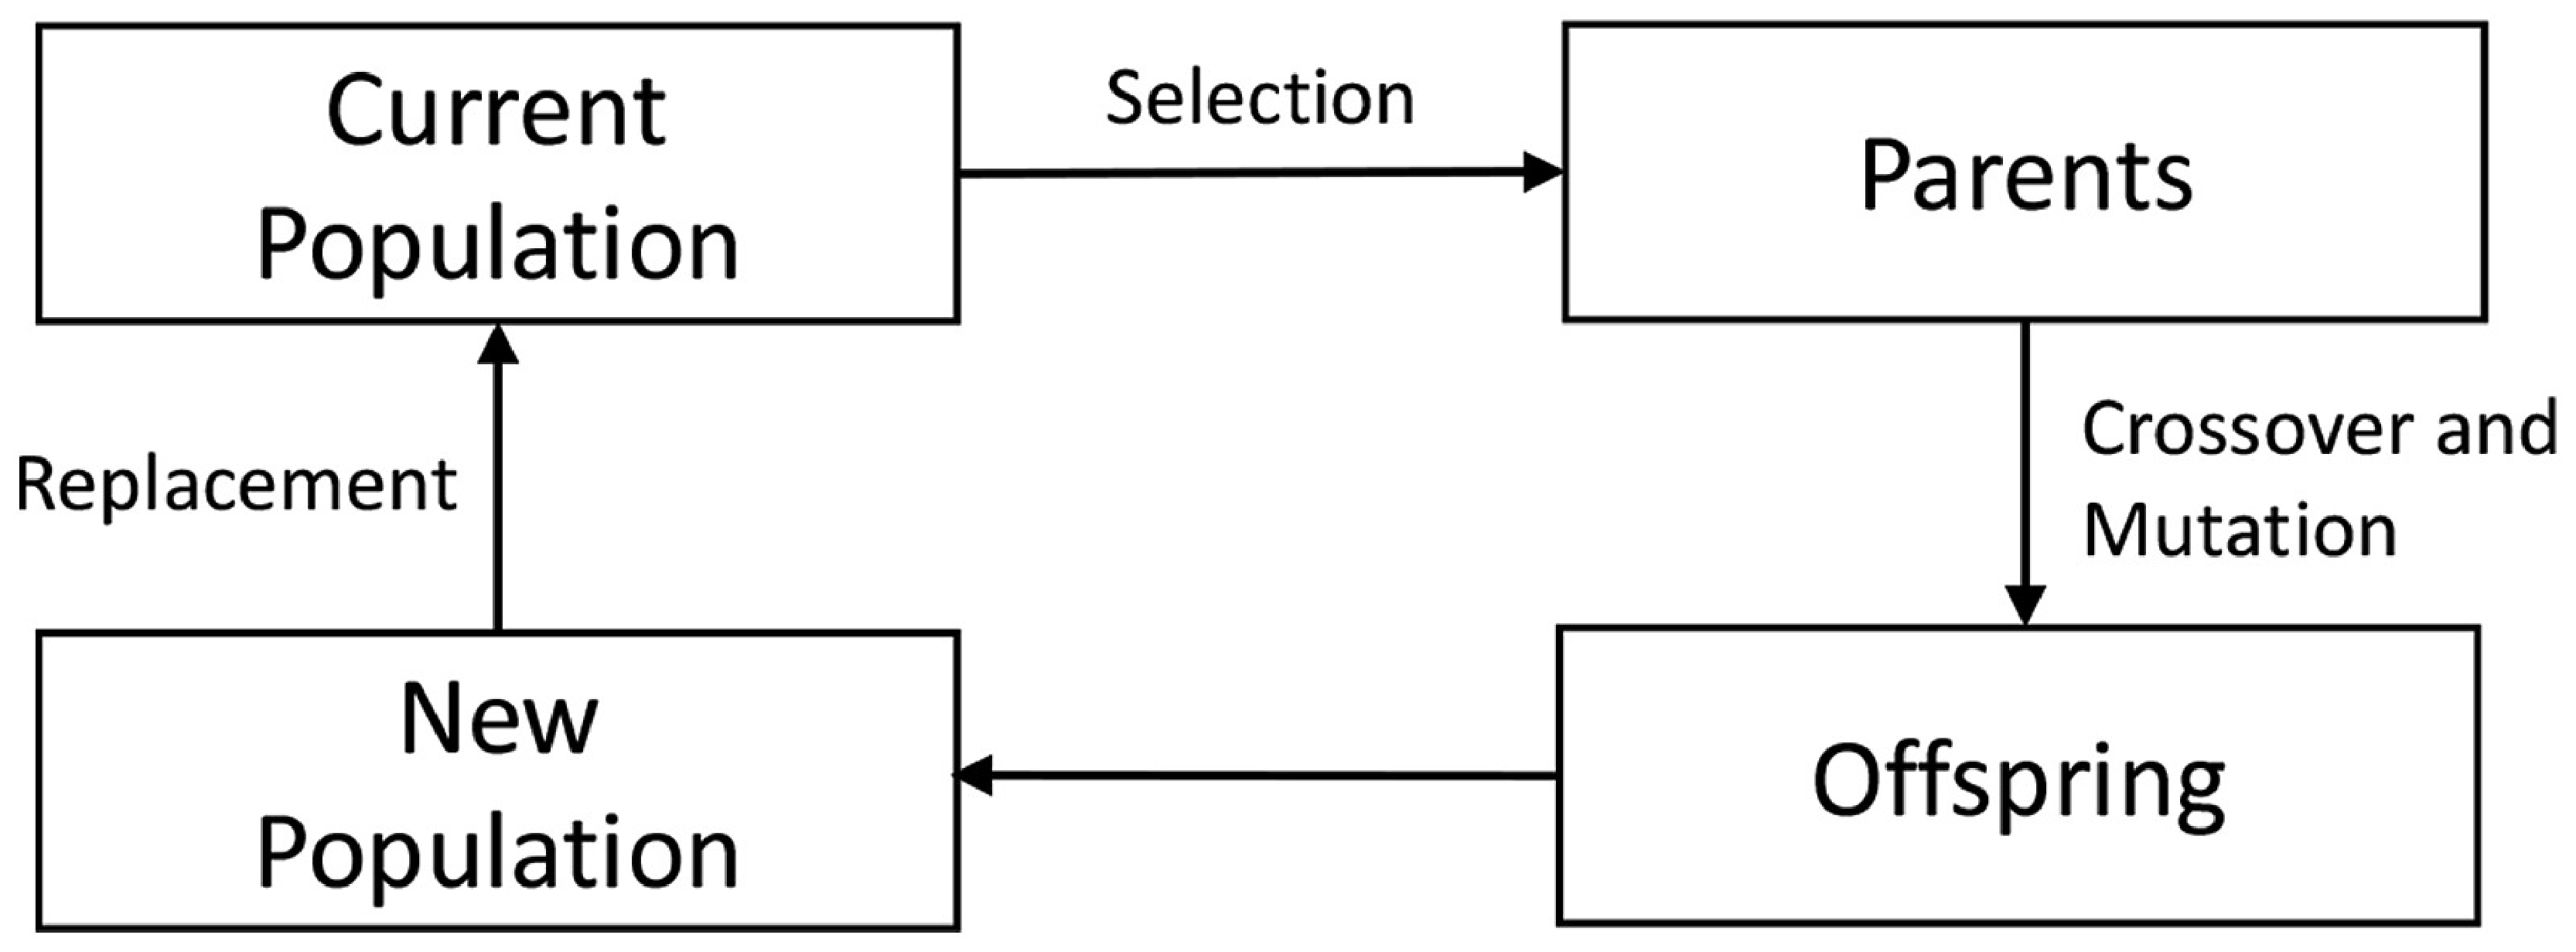
\includegraphics[scale=0.22]{figs/gen-algo.eps}
     \caption{Genetic algorithm optimization loop.}\label{Fig:PROGAN}
 \end{figure}


\noindent Standard genetic algorithm uses several operators for optimization purposes:

% Crossover is a process in which members of the last population are mated at random in the mating pool. So, a pair of offsprings is generated, combining elements from two parents (members), which hopefully have improved fitness values. Mutation is the occasional (with small probability) random alteration of the value of a string position. In fact, mutation is a process of random walk through the coded parameter space. Its purpose is to ensure that important information contained within strings may not be lost prematurely.

% Crossover operators may work for both intensification and diversification during the search, depending on the type of crossover operator and the locations of parents with respect to each other.

% Mutation operators is generally regarded as a random disturbance term of the individual chromosome, such that it can escape from the local area. 

% Uniform mutation that replaces the value of a decision variable by a uniformly distributed random number between the variable lower and upper bounds (R2 = random number in [x2l, x2u]). Example outcome of (c) single-point crossover and (d) uniform mutation in a 2D decision variable space.

% Mutation works to preserve and introduce diversity during the search. It enables the EA to escape local optima.

\begin{enumerate}
\item \textbf{Crossover} - process in which units from latest population are \textit{mixed} together at random. In this way, offsprings that come from the parents have combined features from both parents. It works for intensification and diversification of search, although it depends on the type of crossover operator and the location of the parents in the search space.
\item \textbf{Mutation} - these operators are widely regarded as introducing some random disturbance for individual units in the population. Uniform mutation replaces the value of a single decision variable by a value that is randomly selected from a space within lower and upper bound for given variable. This mainly introduces diversification and also helps to escape local optima.
\item \textbf{Replacement} - after performing crossover and mutation for given population, newly generated offspring are evaluated by the fitness function. Several (this number is usually dependent on the algorithm hyperparameters) newly created members with best score are placed in the population, the same number of worst units is removed.
\item \textbf{Selection} - the most promising units from population (members with best results regarding the fitness function) are chosen for mating. This generally promises the best chance to generate better units in the next population.
\end{enumerate}


 \begin{figure}[ht!]
     \centering
     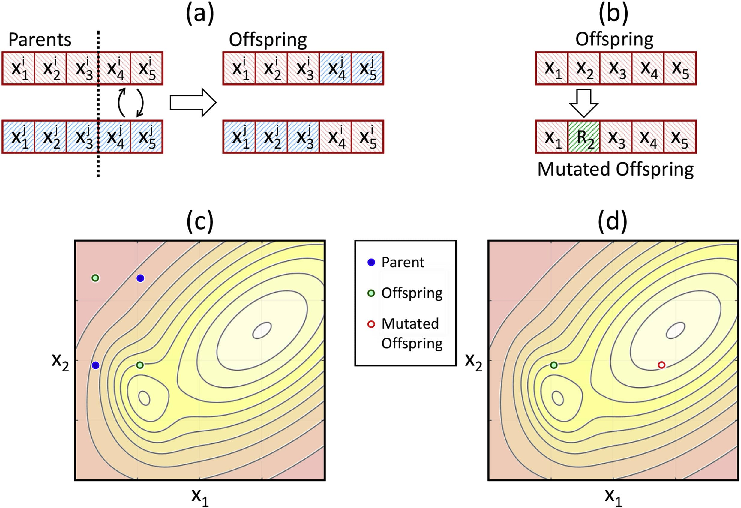
\includegraphics[scale=0.17]{figs/gen-algo-2.eps}
     \caption{Example of crossover and mutation operations.}\label{Fig:PROGAN}
 \end{figure}
 
The algorithm terminates based on several common criteria, most often when a solution is found that satisfies minimum criteria or when fixed number of generations is reached. Below is the pseudocode for the base genetic algorithm. 

 \begin{figure}[ht!]
     \centering
     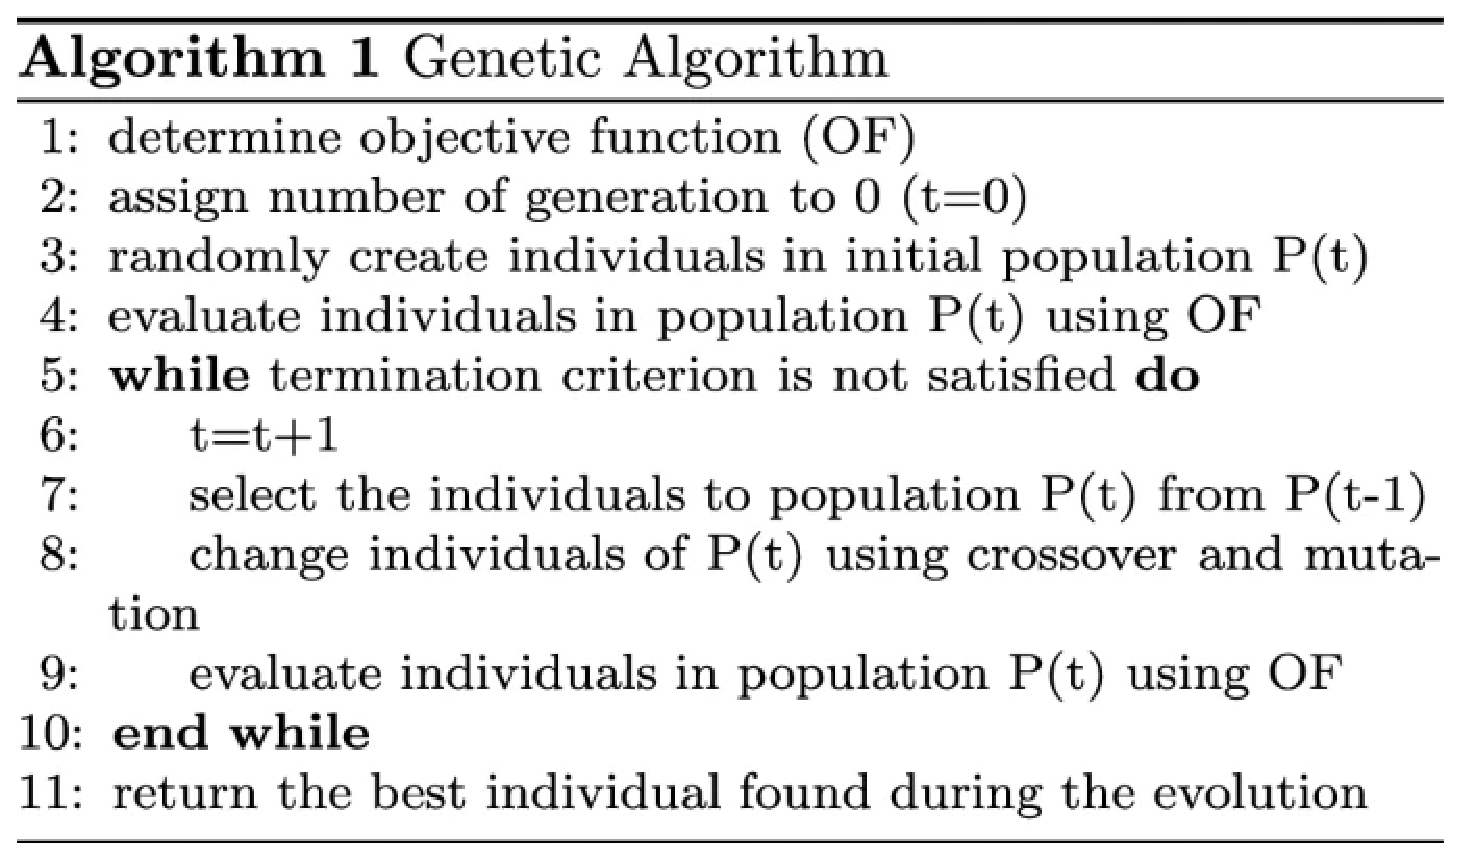
\includegraphics[scale=0.4]{figs/gen-algo-pseudo.eps}
     \caption{Genetic algorithm pseudocode.}\label{Fig:PROGAN}
 \end{figure}

% 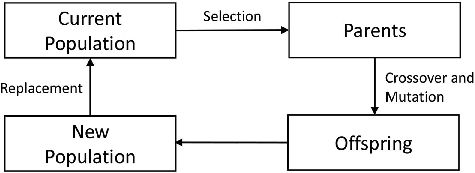
\includepdf[scale=0.5]{figs/gen-algo.pdf}

% The genetic algorithm (GA) [1] is one of the oldest and most known optimization techniques, which are based on nature. In the GA, the search for solution space imitates the natural process which takes place in the environment, and the Darwinian theory of species evolution is taken into consideration. In GAs, we have a population of individuals; each, called a chromosome, represents a potential solution to the problem. The problem being solved is defined by the objective function. Depending on how “good” the given individual is fitted to the objective function, the value which represents its quality is attributed to it. This value is referred to as the fitness of the individual, and it is a main evaluating factor. Highly valued individuals have a better chance to be selected to the new generation of the population. In GAs, we have three operators: selection (a new population of individuals is created based on the fitness values of individuals from the previous generation), crossover (typically parts of individuals are exchanged between two individuals selected to the crossover), and mutation (the values of particular genes are changed randomly). Algorithm 1 presents the standard GA in the pseudo-code form (for more details see [7]).

\subsection{Differential Evolution}

Differential evolution algorithm is a very efficient method most commonly used for optimization of function in continuous search space. It was first proposed by Storn and Price in 1995?. 

The main advantages over general genetic algorithm is more efficient memory usage, lower complexity and faster convergence.

 \begin{figure}[ht!]
     \centering
     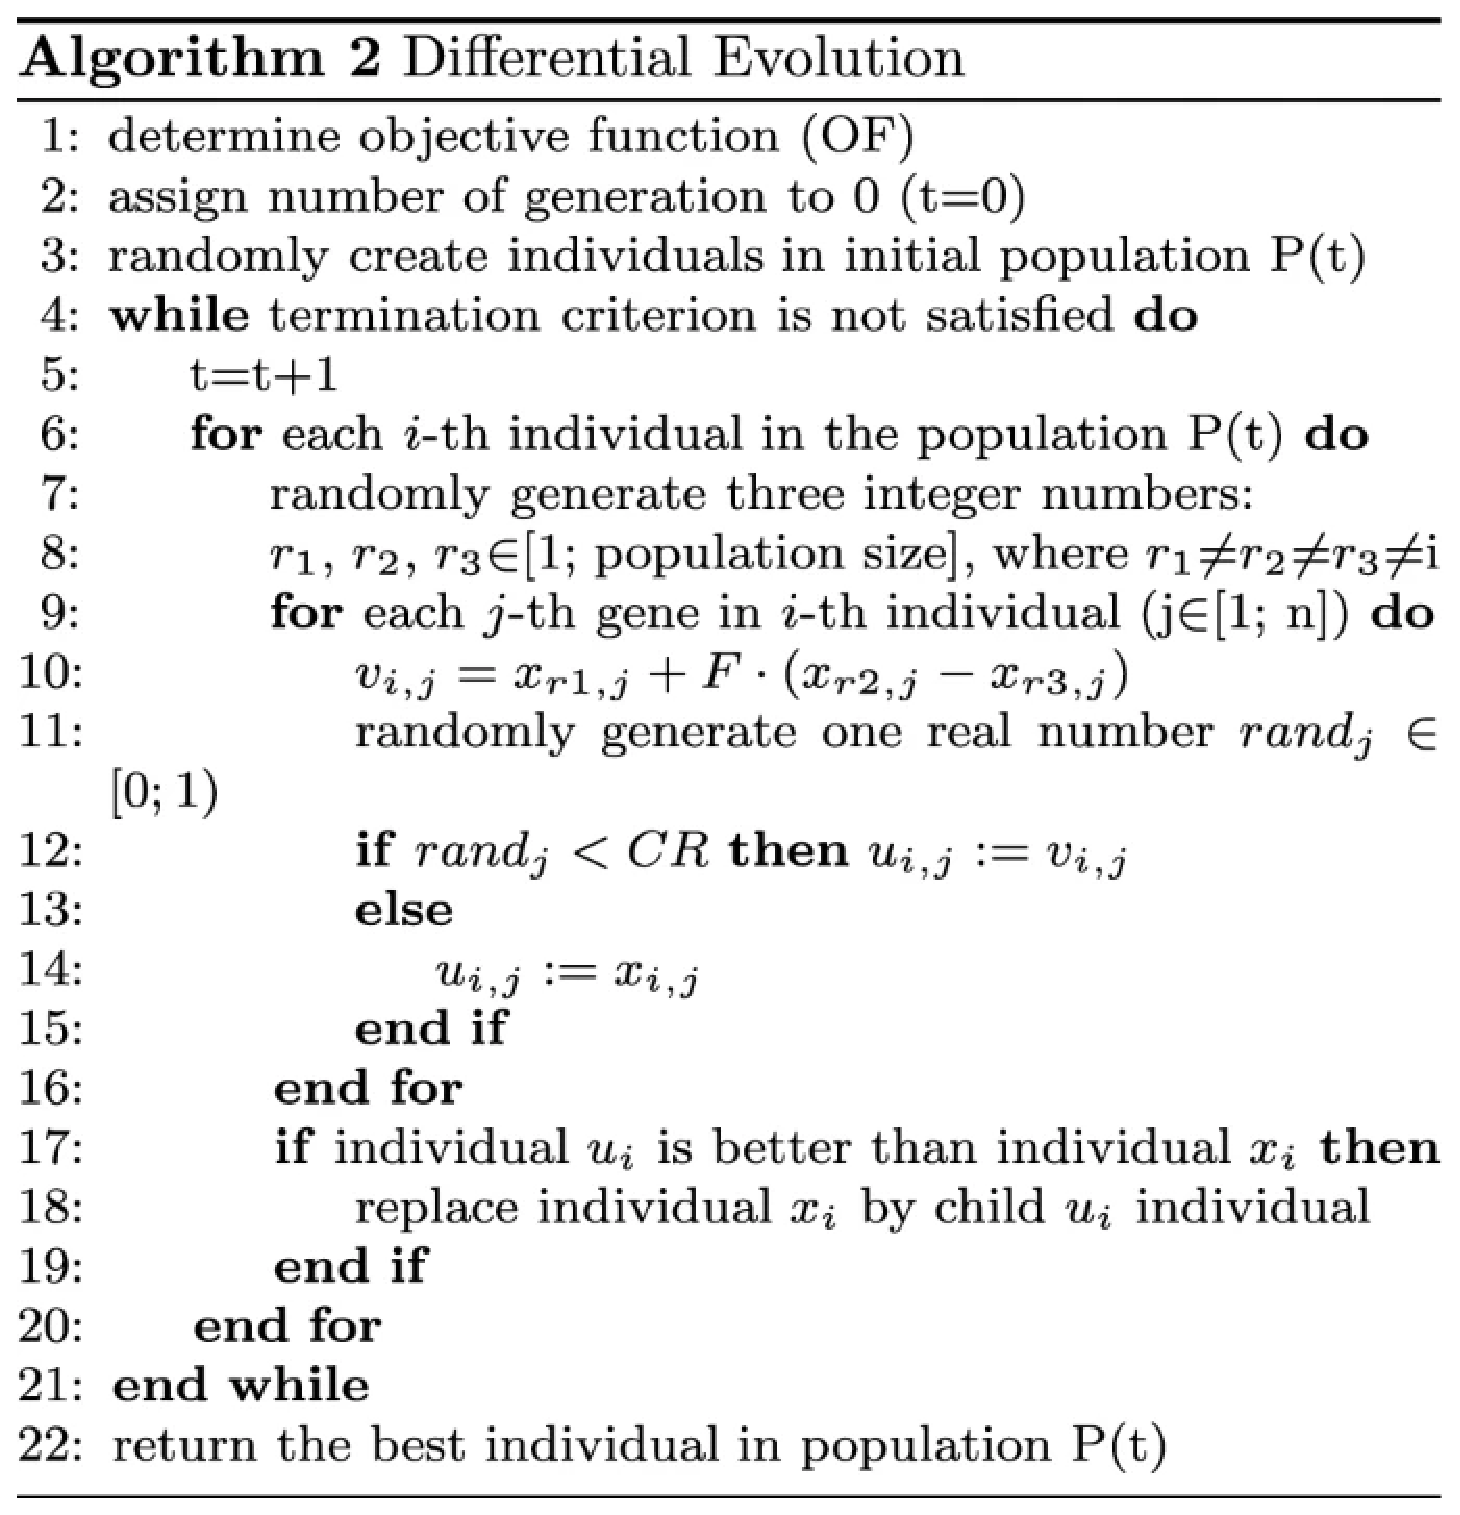
\includegraphics[scale=0.5]{figs/diff-evo.eps}
     \caption{Differential evolution DE/rand/1 pseudocode.}\label{Fig:PROGAN}
 \end{figure}

Below we will present the mathematical formulation of the algorithm and discuss most popular versions.

Differential evolution is primarily described by three parameters: $N_{p}$ - population size, $C_{r}$ - crossover control parameter and $F$ - scaling factor, also known as amplification parameter.\
Each member of every population is described as $D$-dimensional parameter vector. Each population in the algorithm can be understood as vector $\textbf{x}_{i, g}$, where $i \in \{1, 2, ..., N_{p}\}$ and $g$ stands for generation number.

\noindent Method incorporates usage of three vectors, which we will name for simplicity:

\begin{itemize}
\item Donor vector, which is created in the mutation step,
\item Trial vector, which is created in the crossover step,
\item Target vector, which is the vector of current population.
\end{itemize}


In the \textbf{mutation} step donor vector $v_{i, g}$ is produced. It is calculated by adding the scaled difference of two vectors to the third vector from the population. There are two most popular variations of mutation used in differential algorithm, one is the \textit{DE/rand/1} version, where all three vectors used in mutation are taken at random, which allows us to write a formula for donor vector  $v_{i, g}$ as

\begin{equation}
\mathbf{v}_{i, g}=\mathbf{x}_{r_{1}, g}+F\left(\mathbf{x}_{r_{2}, g}-x_{\mathbf{r}_{3}, g}\right),
\end{equation}

\noindent where $r_{1}, r_{2},r_{3} \in \{1, 2, ..., N_{p}\}$ are randomly selected indices and $F$ is the aforementioned scaling factor.

The other choice is the \textit{DE/best/1} version, which chooses two random vectors to calculate the scaled value which is used to change the \textbf{best} vector $\mathbf{x}_{best, g}$ in current population, which results in more greedy version of the method

\begin{equation}
\mathbf{v}_{i, g}=\mathbf{x}_{best, g}+F\left(\mathbf{x}_{r_{2}, g}-x_{\mathbf{r}_{3}, g}\right).
\end{equation}

After the mutation algorithm performs \textbf{crossover} step. There are two most popular crossover schemes: binomial and exponential. Crossover step is performed using rate parameter $C_{r} \in \left(0, 1\right)$, which determines size of perturbation of the target vector. This influences the population diversity.\\
\indent In binomial crossover, the trial vector $\mathbf{u}_{i, g}=\left(u_{i, 1, g}, u_{i, 2, g}, \ldots, u_{i, D, g}\right)$ for $i \in \{1, 2, ..., N_{p}\}$ and $j \in \{1, 2, ..., D\}$ is created using formula

\begin{equation}
u_{i, j, g}=\left\{\begin{array}{ll}
v_{i, j, g} & \text{if } rand_{j} \leqslant C_{r} \text { or } j=j_{\mathrm{rd}}, \\
x_{i, j, g} & \text { otherwise,}
\end{array}\right.
\end{equation}

\noindent where $rand_{j}$ is a random number from $(0,1)$ which determines the probability that the $j$-th parameter will crossover and $\mathbf{v}_{i, g}$ is the donor vector calculated in the mutation step. Also, $j_{\mathrm{rd}}$ is a randomly chosen integer in the range $[1, D]$, which ensures that at least one parameter will be chosen for crossover. That ensures that the new population will be always different from previous one.\

For exponential crossover scheme, let us define the indices $a$ and $b$ to be chosen independently and at random from $[1, D]$. These parameters are chosen for each trial vector separately. Let's denote $\left(\right)_{MOD_{D}}$ as modulo function with modulus $D$. Using these we can define a set of indices
\begin{equation}
I = \left\lbrace a, \left(a+1\right)_{MOD_{D}}, \ldots, \left(a+b-1\right)_{MOD_{D}}\right\rbrace.
\end{equation}
The trial vector $\mathbf{u}_{i, g}=\left(u_{i, 1, g}, u_{i, 2, g}, \ldots, u_{i, D, g}\right)$ for $i \in \{1, 2, ..., N_{p}\}$ and $j \in \{1, 2, ..., D\}$ is created as
\begin{equation}
u_{i, j, g}=\left\{\begin{array}{cc}
v_{i, j, g} & \text {if } j \in I \text { and } rand_{j} \leqslant C_{r}, \\
x_{i, j, g} & \text { otherwise. }
\end{array}\right.
\end{equation}

\noindent Essentially, above formula is focusing on the crossover between neighbouring vector features instead of fully randomizing the choice.\\
Having produced a trial vector we can proceed to the selection step. In this phase, algorithm is greedily choosing new members of the population using the \textit{fitness function} $f$.

\begin{equation}
\mathbf{x}_{i+1, g}=\left\{\begin{array}{ll}
\mathbf{u}_{i, g} & \text {if } f\left(\mathbf{u}_{i, g}\right)<f\left(\mathbf{x}_{i, g}\right), \\
\mathbf{x}_{i, g} & \text { otherwise }
\end{array}\right.
\end{equation}

The algorithm terminates on similar basis as genetic algorithm discussed previously, when a optimal solution below certain treshold is found or when algorithm reaches some defined number of generations.


%
%Crossover: DE crossover strategies control the
%number of inherited components from the mutant
%vector to form a target vector. Binomial and exponential are main crossover schemes 16, 31. The
%DE crossover rate parameter Cr
%influences the size
%of the perturbation of the base (target) vector to
%ensure the population diversity 17
%.
%Binomial crossover: In the crossover operation
%of DE algorithm, a trial vector is formed. In the
%binomial crossover scheme, the trail vector ui,g =
%〈ui,1,g
%, ui,2,g
%, . . . , ui,D,g
%〉 is generated by the equation,
%for i = 1, 2, . . . ,Np
%, j = 1, 2, . . . , D


%
%DE algorithm has three different parameters: a
%population of size Np
%, a crossover control parameter
%Cr
%, and a difference vector amplification parameter
%F. Each population member in DE is represented
%as a D-dimensional parameter vector. In DE algorithm, the population is initialized randomly and is
%supposed to cover the entire search space. Each
%vector in the DE is represented by xi,g
%, where i =
%1, 2, 3, . . . ,Np and g is generation number. New
%offsprings in DE algorithm are generated by mutation, crossover, and selection operators. The repair
%operator proposed by Wang 30 is also used in th
%




%
%source:
%Storn, R., and Price, K. (1995). Differential Evolution—A Simple and Efficient Adaptive Scheme for Global Optimization Over Continuous Spaces. Technical Report, Berkeley, CA. Available online at: https://www.icsi.berkeley.edu/ftp/global/global/pub/techreports/1995/tr-95-012.pdf

% Differential evolution [3, 4], or DE, is a relatively recent EA formulation which uses a mechanism for
% adaptive search that does not make use of probability distributions. Whilst its basic mechanism is
% similar to a GA, its mutation operator is quite different, using a geometric approach that is motivated
% by the moves performed in the Nelder Mead simplex search method. This involves selecting two
% existing search points from the population, taking their vector difference, scaling this by a constant F,
% and then adding this to a third search point, again sampled randomly from the population. Following
% mutation, DE’s crossover operator recombines the mutated search point (the mutant vector) with
% another existing search point (the target vector), replacing it if the child solution (known as a trial
% vector) is of equal or greater objective value. There are two standard forms of crossover [5]:
% exponential crossover and binomial crossover, which closely resemble GA two-point crossover and
% uniform crossover, respectively. The comparisons between target vector and trial vector play the same
% role as the selection mechanism in a GA or ES. Since DE requires each existing solution to be used
% once as a target vector, the whole population is replaced in the course of applying crossover.
% An advantage of using simplex-like mutations in DE is that the algorithm is largely self-adapting,
% with moves automatically becoming smaller in each dimension as the population converges. More
% generally, the authors of the method have claimed that this sort of self-adaptation means that the size
% and direction of moves are automatically matched to the search landscape, a phenomenon they term
% contour matching. When compared to CMA-ES, for example, this means that the algorithm has few
% parameters and is relatively easy to implement.

%%%The differential evolution (DE) is a type of evolutionary algorithm useful mainly for the function optimization in continuous search space. Although a version of DE algorithm for combinatorial problems has also been discussed [51], the principal version of the DE algorithm was discussed by Storn and Price [3]. The main advantages of DE over a traditional GA are: It is easy to use, and it has efficient memory utilization, lower computational complexity (it scales better when handling large problems), and a lower computational effort (faster convergence) [52]. The standard DE procedure is shown in Algorithm 2. Presented there DE optimizes the problem with n decision variables. Parameter F scales the values added to the particular decision variables (mutation), and CR parameter represents the crossover rate [52] (xi,j is the value of jth decision variable stored in ith individual in the population). More detailed information on how the parameters should be tuned can be found in [53]. The main idea of the DE algorithm is connected with computing the difference between two individuals chosen randomly from the population. (The DE determines the function gradient within a given area—not at a single point.) Therefore, the DE algorithm prevents the solution of sticking at a local extreme of the optimized function [52]. Twenty years of DE development resulted in many modifications. Some of them are shortly presented in Table 1.


% n computational intelligence (CI), an evolutionary algorithm (EA) is a subset of evolutionary computation,[1] a generic population-based metaheuristic optimization algorithm. An EA uses mechanisms inspired by biological evolution, such as reproduction, mutation, recombination, and selection. Candidate solutions to the optimization problem play the role of individuals in a population, and the fitness function determines the quality of the solutions (see also loss function). Evolution of the population then takes place after the repeated application of the above operators.

% Evolutionary algorithms are a heuristic-based approach to solving problems that cannot be easily solved in polynomial time, such as classically NP-Hard problems, and anything else that would take far too long to exhaustively process. When used on their own, they are typically applied to combinatorial problems; however, genetic algorithms are often used in tandem with other methods, acting as a quick way to find a somewhat optimal starting place for another algorithm to work off of.
% The premise of an evolutionary algorithm (to be further known as an EA) is quite simple given that you are familiar with the process of natural selection. An EA contains four overall steps: initialization, selection, genetic operators, and termination. These steps each correspond, roughly, to a particular facet of natural selection, and provide easy ways to modularize implementations of this algorithm category. Simply put, in an EA, fitter members will survive and proliferate, while unfit members will die off and not contribute to the gene pool of further generations, much like in natural selection.

% Evolutionary algorithms (EAs) are population-based metaheuristics. Historically, the design of EAs
% was motivated by observations about natural evolution in biological populations. Recent varieties of
% EA tend to include a broad mixture of influences in their design, although biological terminology is
% still in common use. The term ‘EA’ is also sometimes extended to algorithms that are motivated by
% population-based aspects of EAs, but which are not directly descended from traditional EAs, such as
% scatter search. The term evolutionary computation is also used to refer to EAs, but usually as a
% generic term that includes optimisation algorithms motivated by other natural processes, such as
% particle swarm optimisation and artificial immune systems. Although these algorithms often resemble
% EAs, this is not always the case, and they will not generally be discussed in this chapter. For a
% discussion of their commonalities and differences, the reader is referred to [1].
% Over the years, EAs have become an extremely rich and diverse field of study, and the sheer number
% of publications in this area can create challenges to people new to the field. To address this, this
% chapter aims to give a concise overview of EAs and their application, with an emphasis on
% contemporary rather than historical usage.


\chapter{Notable architectures}
\section{StyleGAN}

StyleGAN is an architecture proposed in late 2018 by NVIDIA team. It is considered to be one of the most important publications regarding image generation and it introduces several novelties comparing to models used so far. It used several mechanisms (such as adaptive instance normalization and merging regularization) to generate highly realistic images with great resolution. It is greatly inspired by direct predecessor - Progressive Growing GAN architecture (called ProGAN), also published by NVIDIA.

\begin{figure}[ht!]
    \centering
    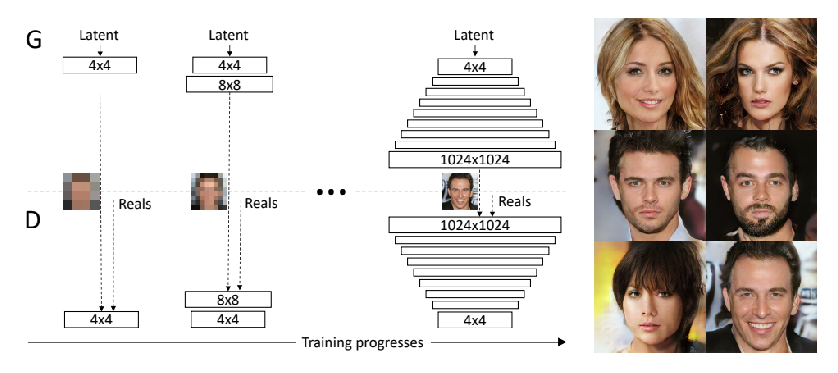
\includegraphics[scale=1.0]{figs/progan-scheme.eps}
    \caption{Progressive growing technique used in ProGAN.}\label{Fig:PROGAN}
\end{figure}

Most important idea presented in the ProGAN architecture, utilized also in StyleGAN, is the progressive structure of learning. Volume of generated by network images is growing from small resolution (starting at 4x4 pixels) to high resolution (up to 1024x1024 pixels) by upsampling. This training principle helps the network to solve simpler task before attending to generate a full-resolution image. It has been proven to help with stability of the training and reduce drastic abnormalities in final image.

\subsection{Architecture overview}

\begin{figure}[ht!]
    \centering
    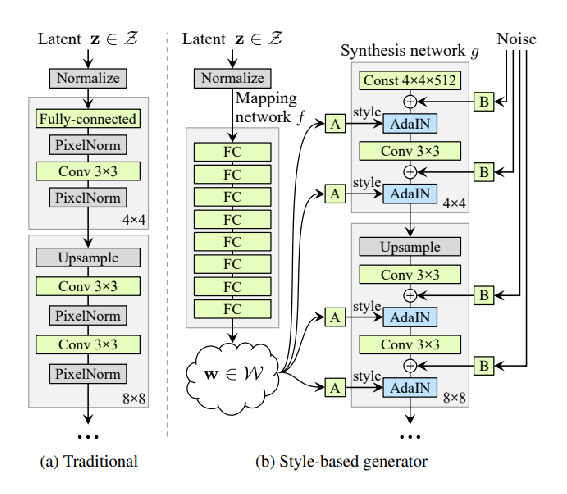
\includegraphics[scale=1.5]{figs/stylegan-scheme.eps}
    \caption{ProGAN and StyleGAN networks comparison.}\label{Fig:STYLEGAN}
\end{figure}


FULL OVERVIEW OF ARCHITECTURE (FULL BUILD, LAYERS, PARAMETERS ITD.) HERE.ALSO DATASET IT WAS TRAINED ON.

TALK ABOUT CONVOLUTIONS MAYBE, SOME GENERAL STUFF NOT TO ATTACK WITH ALL THE FANCY SMART TALK.

SAME FOR OTHER ARCHITECTURES, stylegan2 and biggan.

\subsection{Mapping network}

In the StyleGAN architecture authors introduced a intermediate layer between an input (latent vector $z \in \mathbb{Z}$) and the network called mapping layer (fig...). It works by applying 8 fully connected layers to the input and therefore encoding it as a new vector $w \in \mathbb{W}$. Main purpose of this procedure is to have better control over generative power of the model by separating elements of the vector that will be responsible for different image features.


\begin{figure}[ht!]
    \centering
    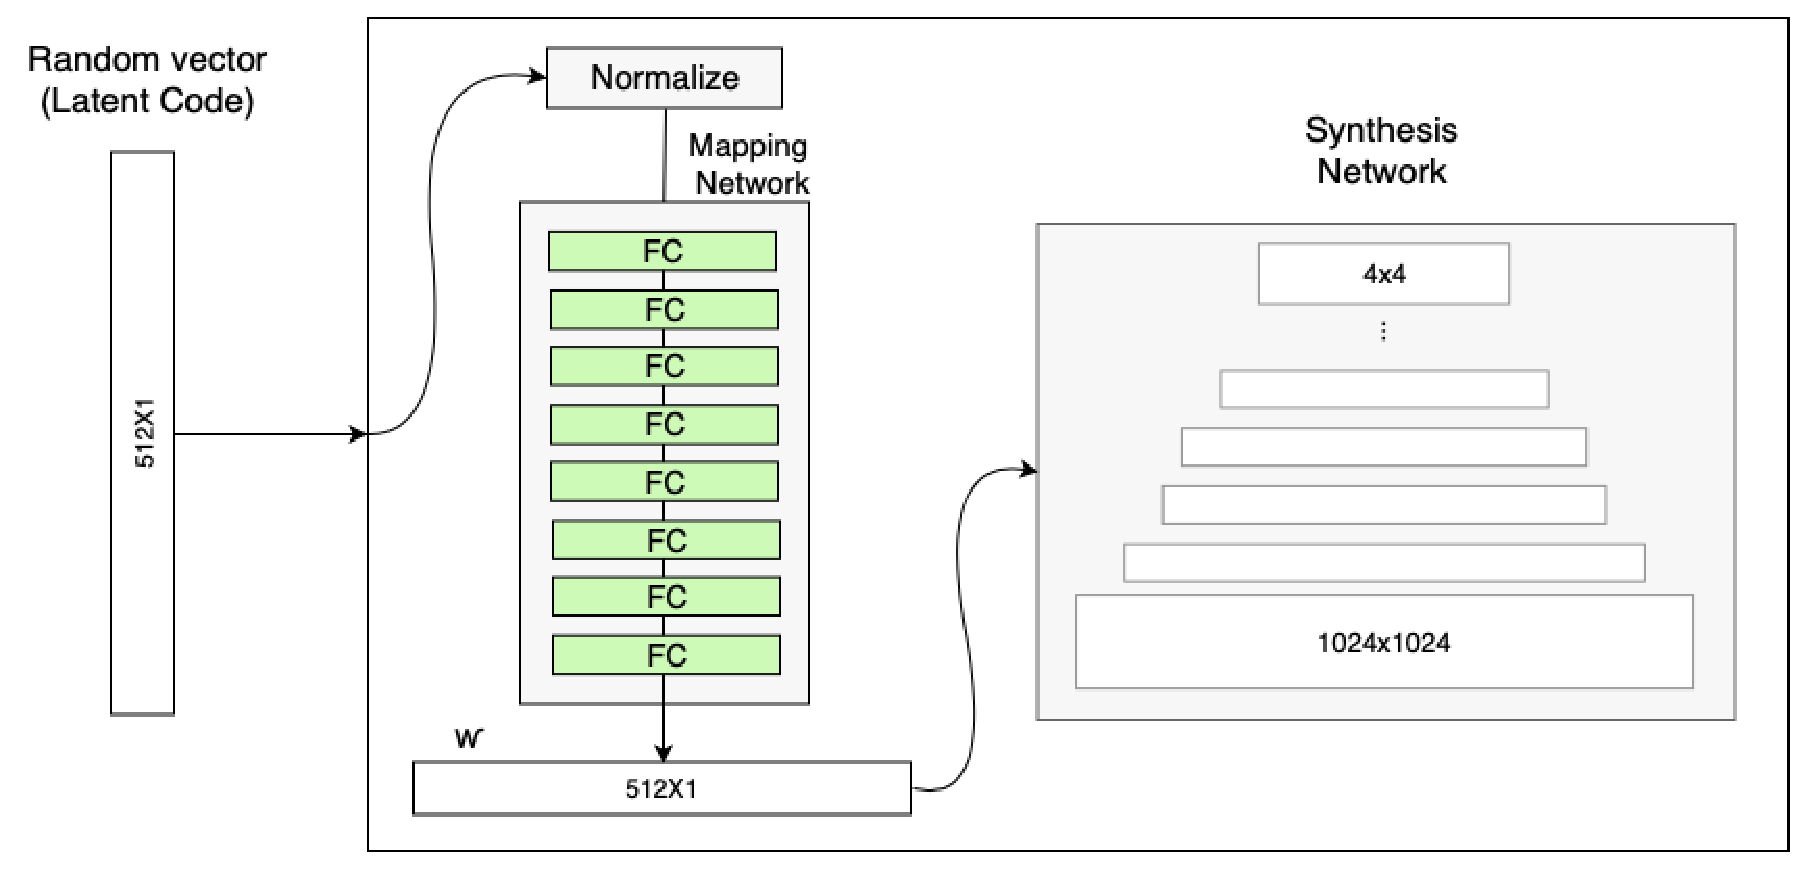
\includegraphics[scale=0.3]{figs/mapping-network.eps}
    \caption{Mapping network of StyleGAN.}\label{Fig:STYLEGAN}
\end{figure}


A common problem for generative models is a phenomenon called \textbf{feature entanglement}. We can consider a scenario where training is done on a dataset of human faces. It is very likely that most of the women in the dataset will have long hair and most men - short hair. This would result in the entanglement of \textit{hair length} and \textit{gender} features. Therefore, when latent vector is manipulated in order to change the hair length - the model will also change the gender of a person on the image, as it is associating these two occurencies as bounded together. The mapping layer is separating these features, allowing to change different elements of new vector $w$ without losing the integrity of an image.

\subsection{Adaptive Instance Normalization}

% https://arxiv.org/pdf/1703.06868.pdf - paper
% https://arxiv.org/pdf/1607.08022.pdf%7B - fast style transfer paper
% https://www.coursera.org/lecture/build-better-generative-adversarial-networks-gans/adaptive-instance-normalization-adain-cr6bv - explained
% https://towardsdatascience.com/light-on-math-machine-learning-intuitive-guide-to-neural-style-transfer-ef88e46697ee - style transfer

In the traditional generator, latent code is introduced to the network only in the first layer. The authors of StyleGAN are using the vector $w$ produced via mapping network to steer the style of an image at each convolutional layer by using \textbf{Adaptive Instance Normalization (AdaIN)} technique.

% HERE THE EQUATION FOR ADAIN
\begin{figure}[ht!]
    \centering
    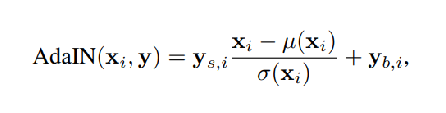
\includegraphics[scale=1.2]{figs/adain.eps}
    \caption{Mapping network of StyleGAN.}\label{Fig:STYLEGAN}
\end{figure}

The middle part of the equation is the \textbf{Instance Normalization (IN)}. Each channel of the convolution layer is normalized. Values $\textbf{y}_{s,i}$ and $\textbf{y}_{b,i}$ are calculated from the vector $v$ using fully-connected layer and correspond to \textit{A} on the figure-main one. These can be understood as scale and bias; these values are used to translate the information from vector $w$ to a feature map generated by convolution.

\begin{figure}[ht!]
    \centering
    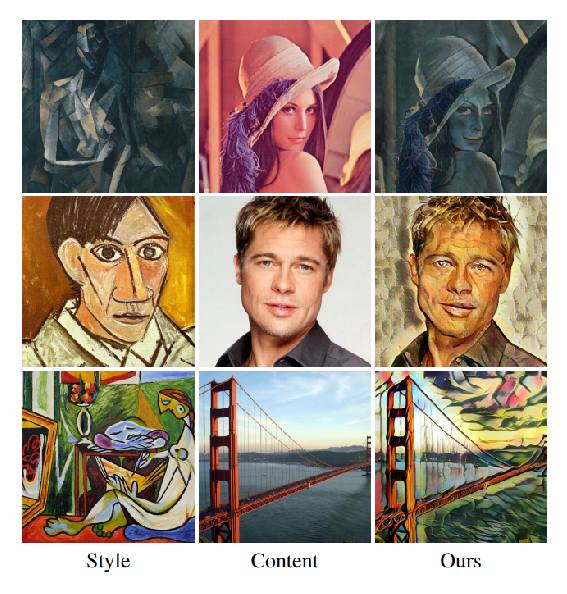
\includegraphics[scale=1.0]{figs/adaptive-instance-norm.eps}
    \caption{Example of AdaIN application for style transfer.}\label{Fig:STYLEGAN}
\end{figure}

Adding this method of including latent vector at every step of network computation resulted in drastic improvement of network's performance which can be see in the table below.

\begin{figure}[ht!]
    \centering
    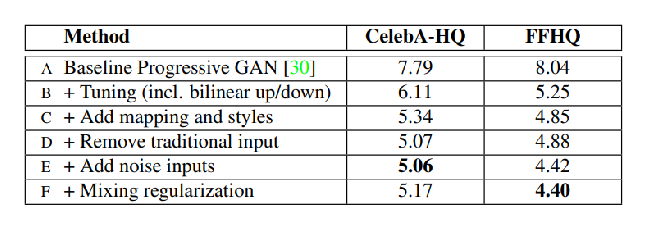
\includegraphics[scale=1.2]{figs/frechet-distance.eps}
    \caption{Mapping network of StyleGAN.}\label{Fig:STYLEGAN}
\end{figure}


%%%% NOTES %%%%

% This normalization is called \textit{adaptive}, because 

% Main task of this structure is elastic 

% where the input feature map is normalized with instance normalization first. Then, StyleGAN scales and biases each normalized spatial feature map by the style information. (μ and σ are the mean and the standard deviation of the input feature map xᵢ respectively.) In each layer, StyleGAN computes a pair of style values (y(s, i) and y(b, i)) as the scale and the bias from w to apply the style to the spatial feature map i. The normalized feature influences the amount of style applied to a spatial location.


% The AdaIN (Adaptive Instance Normalization) module transfers the encoded information ⱳ, created by the Mapping Network, into the generated image. The module is added to each resolution level of the Synthesis Network and defines the visual expression of the features in that level:
% Each channel of the convolution layer output is first normalized to make sure the scaling and shifting of step 3 have the expected effect.
% The intermediate vector ⱳ is transformed using another fully-connected layer (marked as A) into a scale and bias for each channel.
% The scale and bias vectors shift each channel of the convolution output, thereby defining the importance of each filter in the convolution. This tuning translates the information from ⱳ to a visual representation.


% While a traditional generator [30] feeds the latent code
% though the input layer only, we first map the input to an intermediate latent space W, which then controls the generator
% through adaptive instance normalization (AdaIN) at each convolution layer. Gaussian noise is added after each convolution, before evaluating the nonlinearity. Here “A” stands for a learned
% affine transform, and “B” applies learned per-channel scaling factors to the noise input. T



% Mapping Network
% The Mapping Network’s goal is to encode the input vector into an intermediate vector whose different elements control different visual features. This is a non-trivial process since the ability to control visual features with the input vector is limited, as it must follow the probability density of the training data. For example, if images of people with black hair are more common in the dataset, then more input values will be mapped to that feature. As a result, the model isn’t capable of mapping parts of the input (elements in the vector) to features, a phenomenon called features entanglement. However, by using another neural network the model can generate a vector that doesn’t have to follow the training data distribution and can reduce the correlation between features.
% The Mapping Network consists of 8 fully connected layers and its output ⱳ is of the same size as the input layer (512×1).

% Mapping Network moreover Style Network: The purpose of the mapping network is to produce the latent input vector within the intermediate vector whose distinctive element control various visual features. Instead of immediately implementing latent vector to the input layer, mapping is done.

% The main principle behind training the StyleGAN is this “progressive” method which was first used by NVIDIA in their ProGAN. It works by gradually increasing the resolution , thus ensuring that the network evolves slowly, initially learning a simple problem before progressing to learning more complex problems(or, in this case, images of a higher resolution). This kind of training principle ensure stability and has been proven to minimize common problems associated with GANs such as mode collapse. It also makes certain that high level features are worked upon first before moving on to the finer details, reducing the likelihood of such features being generated wrong(which would have a more drastic effect on the final image than the other way around). StyleGANs use a similar principle, but instead of generating a single image they generate multiple ones, and this technique allows for styles or features to be dissociated from each other.

% Baseline Progressive Growing GANs: Style GAN uses baseline progressive GAN structure, which means the volume of the generated picture increases progressively from a shallow resolution (4×4) to high resolution (1024 x1024) by adding a new section to both the models to maintain the larger resolution after applying the model on a more modest resolution to make it further stable.

\subsection{Style mixing regularization}

As additional technique of regularization and method to differentiate the generated images further, a \textbf{style mixing} approach was introduced by the authors. The main idea is to use not one but two (or more) latent vectors $w_{1}, w_{2}$ (obtained from mapping of $z_{1}, z_{2}$) to generate the final image. The way in which mixing is introduced is fairly simple; up to certain point in the architecture vector $w_{1}$ is used for style control and from crossover point vector $w_{2}$ is used.
Depending on the place of crossover, final image obtains different characteristics from each image. 

DOPISAĆ DOKŁADNIE ROZMIARY.

\subsection{Additional noise inputs}

Authors provided the generator with ability to alternate very fine details on a picture by adding stochastic variance into the model. Single-channel images of uncorrelated Gaussian noise are fed into different places in the architecture. Noise is scaled per channel (which means that the amount of noise is a learnable parameter) and added after each convolution layer before AdaIN layer.

\begin{figure}[ht!]
    \centering
    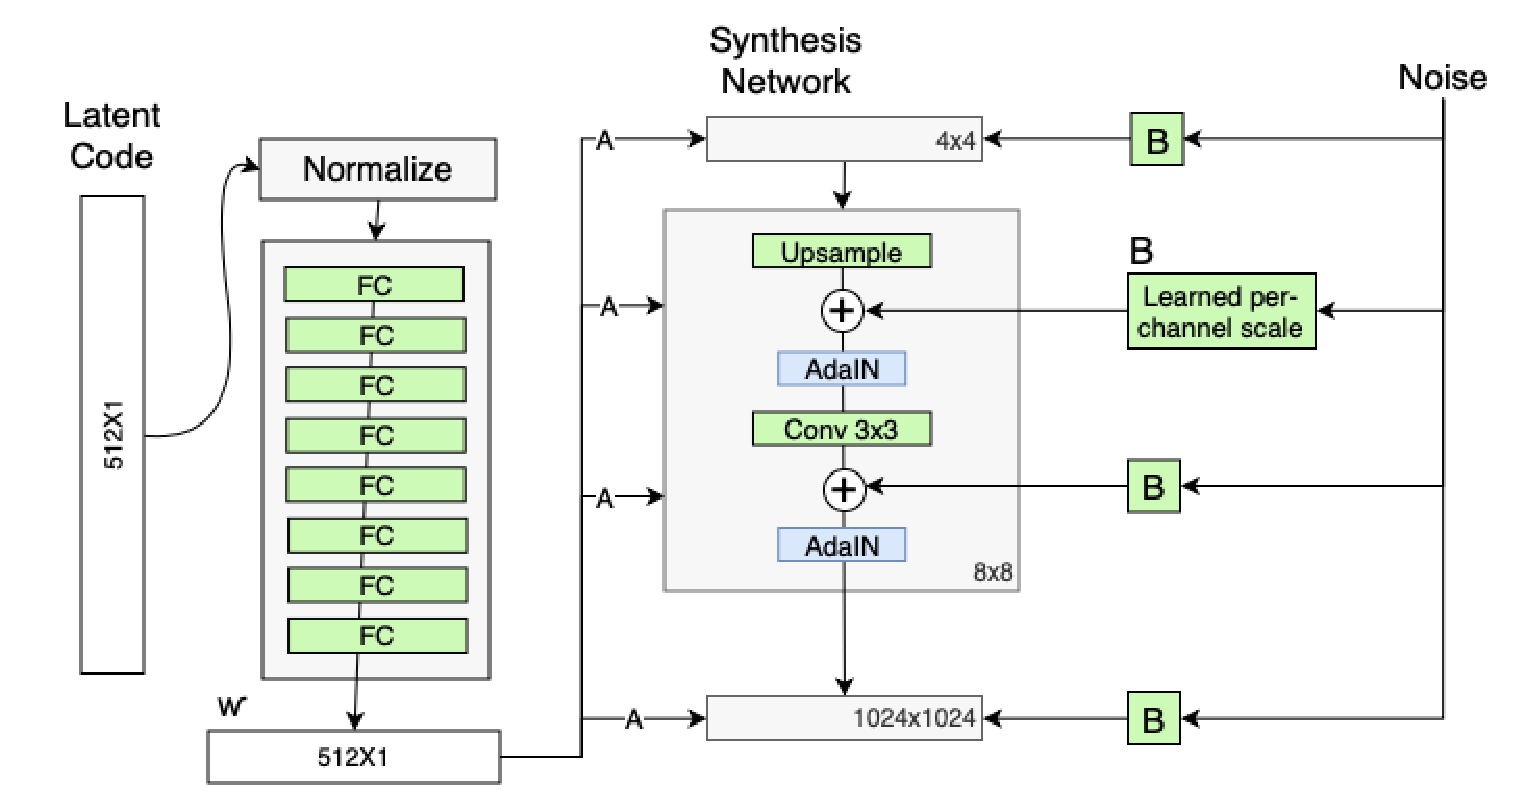
\includegraphics[scale=0.5]{figs/noise.eps}
    \caption{Places in the architecture where noise is added.}\label{Fig:STYLEGAN}
\end{figure}

Additional noise allows to generate and alternate very detailed parts of the image (wrinkles, freckles, hair). Thanks to scalability and DOKONCZYC

\begin{figure}[ht!]
    \centering
    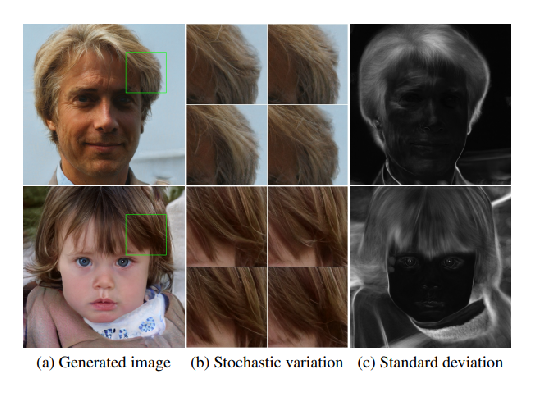
\includegraphics[scale=1.4]{figs/stochastic-variation.eps}
    \caption{Visual inspection of where the gaussian noise tends to be the most active.}\label{Fig:STYLEGAN}
\end{figure}

% Gaussian noise is added after each convolution, before evaluating the nonlinearity. Here “A” stands for a learned
% affine transform, and “B” applies learned per-channel scaling factors to the noise input.

% Finally, we provide our generator with a direct means
% to generate stochastic detail by introducing explicit noise
% inputs. These are single-channel images consisting of uncorrelated Gaussian noise, and we feed a dedicated noise
% image to each layer of the synthesis network. The noise
% image is broadcasted to all feature maps using learned perfeature scaling factors and then added to the output of the
% corresponding convolution, as illustrated in Figure 1b. The
% implications of adding the noise inputs are discussed in Sections 3.2 and 3.3.


% There are many aspects in people’s faces that are small and can be seen as stochastic, such as freckles, exact placement of hairs, wrinkles, features which make the image more realistic and increase the variety of outputs. The common method to insert these small features into GAN images is adding random noise to the input vector. However, in many cases it’s tricky to control the noise effect due to the features entanglement phenomenon that was described above, which leads to other features of the image being affected.
% The noise in StyleGAN is added in a similar way to the AdaIN mechanism — A scaled noise is added to each channel before the AdaIN module and changes a bit the visual expression of the features of the resolution level it operates on.


\section{StyleGAN2}

Significant improvements of the StyleGAN architecture were proposed in late 2019. Publication revolved mainly around the problems which emerged during StyleGAN generator. It has been noticed that several parts of the network cause imperfections in the final images, which are called \textit{artifacts}. Two main types of artifacts were formulated in the paper:

\begin{itemize}
\item \textbf{Water-droplet artifacts} - the blob-shaped characteristics that resemble water-droplets are visible in various places in the final images. It might not be obvious while looking at the image, but it is very visible in the intermediate feature maps produced by generator. This artifacts starts to appear around 64x64 pixels resolution and gets stronger with higher resolutions. 
\item \textbf{Phase artifacts} - output images show strong location preference for several features e.g. facial features like teeth or eyes. This causes some of the features to remain unchanged when major components of the image such as pose or rotation are vastly different.
\end{itemize}


\begin{figure}[ht!]
    \centering
    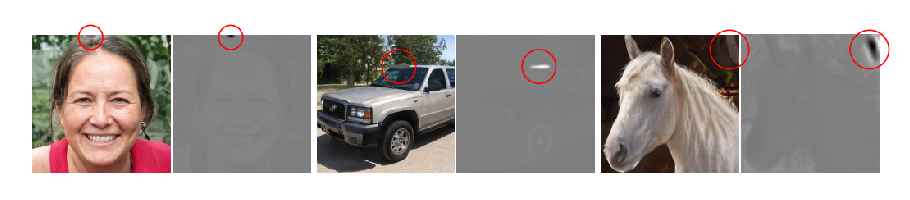
\includegraphics[scale=1.0]{figs/water-droplets.eps}
    \caption{Water droplets artifact and its effect on feature maps.}\label{Fig:STYLEGAN}
\end{figure}



\begin{figure}[ht!]
    \centering
    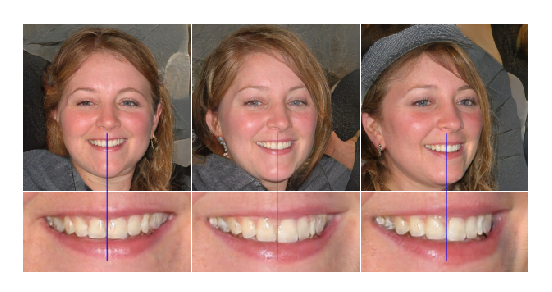
\includegraphics[scale=1.2]{figs/phase.eps}
    \caption{Phase artifact. Blue line helps to visualize that teeth are staying in the same place even with changing a significant feature of image such as rotation of the face..}\label{Fig:STYLEGAN}
\end{figure}

\subsection{Architecture overview}

\begin{figure}[ht!]
    \centering
    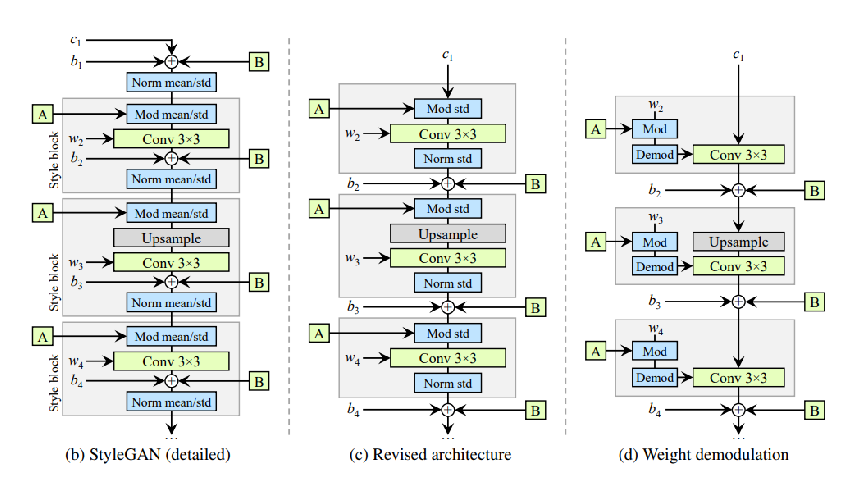
\includegraphics[scale=1.0]{figs/stylegan2-scheme2.eps}
    \caption{Visual inspection of where the gaussian noise tends to be the most active.}\label{Fig:STYLEGAN}
\end{figure}


\subsection{Revisiting Instance Normalization}

The water-droplet effect was speculated to be a side effect of AdaIN method applied in the style blocks. Authors pointed out that this type of normalization affects each feature map separately (works independently for every channel) and potentially destroys meaningful information that is included in the differences between feature maps values.

To address this problem, significant changes to the architecture were proposed.

\begin{figure}[ht!]
    \centering
    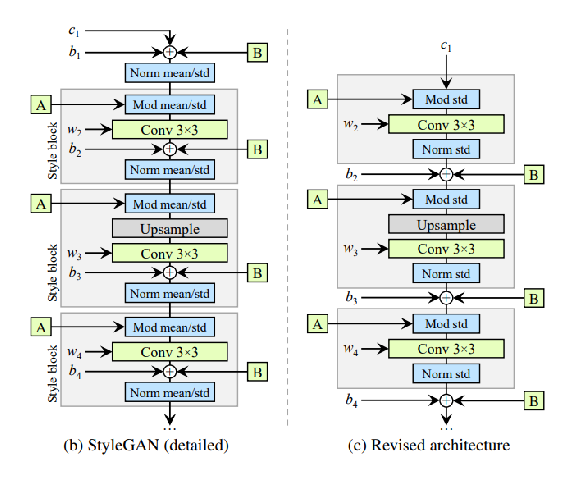
\includegraphics[scale=1.3]{figs/changed-normalization.eps}
    \caption{(b) shows the original StyleGAN architecture. The AdaIN fucntion is shown as combination of normalization and modulation operations. (c) shows the revised model with changes in the network.}\label{Fig:STYLEGAN}
\end{figure}

As seen on the image above, several things changed in the network:

\begin{itemize}
\item Only standard deviation is modified for each feature map, modification of mean was deemed redundant as the effects of this operations were not meaningful for the network. Removing this part made the model simpler,
\item Noise addition was removed from the style block and instead applied inbetween the blocks. This was mainly done to prepare the network for weight modulation,
\item Input vector $c$ is fed to the network directly, without normalization and applying noise.
\end{itemize}

All of these steps were also necessary to introduce the main idea for handling water-droplets artifact problem - \textbf{weight demodulation}.

\begin{figure}[ht!]
    \centering
    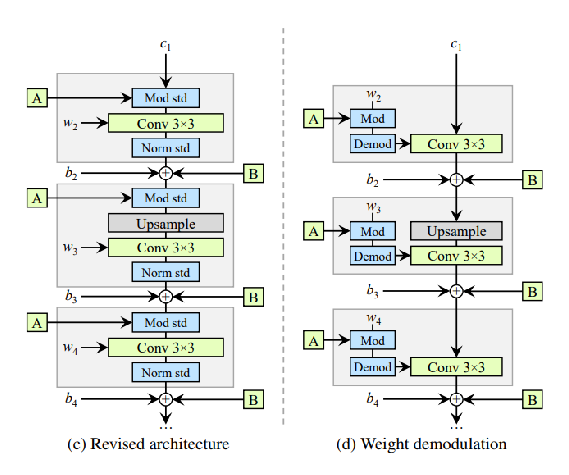
\includegraphics[scale=1.3]{figs/weight-demodulation.eps}
    \caption{(b) shows the original StyleGAN architecture. The AdaIN fucntion is shown as combination of normalization and modulation operations. (c) shows the revised model with changes in the network.}\label{Fig:STYLEGAN}
\end{figure}

HERE WEIGHT DEMODULATION



% First, have constant input(c) directly as model input rather than modified input C with noise and bias.
% Second, the noise and bias are removed from style block and moved outside.
% At last, we only modify standard deviation per feature map rather than both mean and std.

% The authors of StyleGAN2 explain that this kind of normalization discards information in feature maps encoded in the relative magnitudes of activations. The generator overcomes this restriction by sneaking information past these layers which result in these water-droplet artifacts. The authors share the same confusion as the reader as to why the discriminator is unable to distinguish images from this droplet effect.

% StyleGAN2 like StyleGAN uses a normalization technique to infiltrate styles from W vector using learned transform A into the source imagebut now the droplet artifacts are being taken care of. They introduced Weight Demodulation for this purpose. Let us investigate changes made –

\subsection{Removing Progressive Growing}

StyleGAN2 uses different resolution feature maps that are produced in the base network and uses the ResNet like skip connections to incorporate lower resolutions maps to the final output. This change can be viewed as quite drastic - the whole concept of base network was changed, but it proved to be a necessary step in order to mitigate the \textit{phase artifact} effect.


MORE HERE



% StyleGAN2 makes use of the different resolution features maps generated in the architecture and uses skip connections to connect low-res feature maps to final generated image. Bilinear Up/Down-sampling is used within the G and D networks.

% Progressive nature of StyleGAN has attributed to Phase artifacts wherein output images have strong location preference for facial features. StyleGAN2 tries to imbibe the capabilities of progressive growing(training stability for high-res images) and implements a new network design based on skip connection/residual nature like ResNet.

% This new network does not expand to increase image resolution and yet produces the same results. This network is like the MSG-GAN which also uses multiple skip connections. “Multi-Scale Gradients for Generative Adversarial Networks” by Animesh Karnewar and Oliver Wang showcases an interesting way to utilize multiple scale generation with a single end-to-end architecture.


\subsection{Other improvements}

LAZY REGULARIZATION

PATH LENGTH REGULARIZATION

% Main solutions proposed by StyleGAN2

% Eliminating droplet modes by normalizing with estimated statistics instead of AdaIN.
% By using a hierarchical Generator with skip connection (similar to MSG-GAN) instead of Progressive Growing, phase artifacts are reduced.
% Image quality improvement by reducing the Perceptual Path Length (PPL) and smoothing latent space.

% StyleGAN actually generates beautiful and realistic images, but sometimes unnatural parts are generated (artifacts). In the paper "Analyzing and Improving the Image Quality of StyleGAN" these artifacts are exposed and analyzed. Moreover, changes in both model architecture and training methods are proposed to address them.


% We begin by observing that most images generated by
% StyleGAN exhibit characteristic blob-shaped artifacts that
% resemble water droplets. As shown in Figure 1, even when
% the droplet may not be obvious in the final image, it is
% present in the intermediate feature maps of the generator.1
% The anomaly starts to appear around 64×64 resolution,
% is present in all feature maps, and becomes progressively
% stronger at higher resolutions. The existence of such a consistent artifact is puzzling, as the discriminator should be
% able to detect it.
% We pinpoint the problem to the AdaIN operation that
% normalizes the mean and variance of each feature map separately, thereby potentially destroying any information found
% in the magnitudes of the features relative to each other. We



\section{BigGAN}

\chapter{Framework description}

The architecture of solution that we are exploring in this work consists of four main components:
\begin{enumerate}
\item Pre-trained generative model based on Generative Adversarial Network architecture,
\item CLIP model,
\item Evolutionary optimization algorithm,
\item Evaluation using classification network.
\end{enumerate}
Graph below shows the flow of data and describes the overall framework architecture:\\


DOKŁADNIEJ ROZPISAĆ:

\noindent Description of the flowchart:
\begin{enumerate}
\item [1.] First, text is provided by the user,
\item [2.] Introduced text is encoded using pre-trained CLIP model.
\end{enumerate}
Next steps can be considered as a 'optimization loop':
\begin{enumerate}
\item [3a.] Algorithm is performing optimization step,
\item [3b.] Optimized population of samples (vectors)  is serving as an input for generator which produces images,
\item [3c.] Generated images are evaluated by fitness function (in our case, similarity function).
\end{enumerate}
After completing this process, post-processing part takes place:
\begin{enumerate}
\item [4.] Output images are passed for an evaluation using classification network and similarity metric.
\end{enumerate}

We consider StyleGAN2 architecture as the main choice for a generative model in this solution. Main advantages of that choice are:
\begin{itemize}
\item It is widely available as a pre-trained structure; it is public and open-sourced for both generative and discriminative parts of the architecture.
\item It consists of several class-based dedicated models (such as StyleGAN2-car or StyleGAN2-horse). It allows for experimentations with different types of images.
\item It is still considered a state-of-the-art model regarding the quality of produced images and was trained using huge datasets of images.
\end{itemize}

As of optimization algorithm, we used two algorithms described in previous chapters - \textit{genetic algorithm} and \textit{differential evolution}.

% Methodology of a solution:
% In regular 
% Core of this solution consists of using evolutionary algorithm to navigate in the latent space. Thanks to that approach, 


\chapter{Datasets and evaluation}
\chapter{Experiments}
\chapter{Summary}





































%%%% OLD STUFF, MIGHT BE USED FOR FUNCTIONS

% \chapter{Tables and figures}

% Figure \ref{Fig:MV} shows an example of figure and related
% caption.  Do not use too small symbols and lettering in your
% figures.  Warning: your paper will be printed in black and white
% in the proceedings.  You may insert color figures, but it is your
% responsibility to check that they print correctly in black and
% white.  The color version will be kept in the ESANN electronic
% proceedings available on the web.


% Table \ref{Tab:AgeWeight} shows an example of table.

% \begin{table}[ht!]
%   \centering
%   \begin{tabular}{|c|c|c|}
%     \hline
%     ID & age & weight \\
%     \hline
%     1& 15 & 65 \\
%     2& 24 & 74\\
%     3& 18 & 69 \\
%     4& 32 & 78 \\
%     \hline
%   \end{tabular}
%   \caption{Age and weight of people.}\label{Tab:AgeWeight}
% \end{table}



% Poniższa praca dotyczy pewnych własności zmiennych losowych, a zatem wskazane jest przytoczenie pewnych podstawowych definicji z zakresu probabilistyki.

% \begin{df} \textnormal{([3], str. 18)}\*\\
% Trójkę $(\Omega,\mathcal{F},P)$ gdzie $P$ jest funkcją prawdopodobieństwa określoną na $\sigma$-ciele $\mathcal{F}$ podzbiorów zbioru zdarzeń elementarnych $\Omega$, nazywamy przestrzenią probabilistyczną.
% \end{df}

% \begin{df} \textnormal{([3], str. 75)}\*\\
% Funkcję $X: \Omega \rightarrow \mathbb{R}$ nazywamy zmienną losową o wartościach w $\mathbb{R}$, jeżeli dla każdego $a \in \mathbb{R}$ zbiór $X^{-1}((1-\infty,a])$ jest zdarzeniem, czyli $X^{-1}((-\infty,a]) \in \mathcal{F}$.
% \end{df}

% Głównymi zmiennymi losowymi rozważanymi w tej pracy będą ciągłe zmienne losowe zdefiniowane następująco:

% \begin{df} \textnormal{([1], str. 31)}\*\\
% Mówimy, że zmienna losowa X jest typu ciągłego, jeżeli istnieje nieujemna funkcja f, określona i 
% całkowalna do jedynki na całej osi, spełniająca warunek 
% \begin{center}
% $\forall_{[x_{1}, x_{2}]} \: P\left(\left\lbrace\omega: x_{1} \leqslant X(\omega) \leqslant x_{2}\right\rbrace\right) = \int\limits^{x_2}_{x_1} f(x)dx.$
% \end{center}
% \end{df}

% \begin{df} \textnormal{([1], str. 35)}\*\\
% Niech $p \in (0,1)$. Liczbę $q_{p}(X)$ spełniającą warunki:

% \begin{center}
% $P(X \leqslant q_{p}(X)) \geqslant p \wedge P(X < q_{p}(X)) \leqslant p$
% \end{center}

% nazywamy kwantylem rzędu $p$ zmiennej losowej $X$.
% \end{df}

% \noindent Kwantyle tego samego rzędu tworzą przedział $[q^{-}_{X}(p),q^{+}_{X}(p)]$ gdzie
% \begin{gather}
% \begin{split}
% q^{-}_{X}(p) &=\textnormal{sup}\{x: P(X<x)<p\} \\ \nonumber
% 								 &=\textnormal{inf} \{x: F(x)\geqslant p \} \nonumber
% \end{split}
% \end{gather}
% oraz\
% \begin{gather}
% \begin{split}
% q^{+}_{X}(p) &=\textnormal{inf}\{x: F(x)>p\} \\ \nonumber
% 								 &=\textnormal{sup} \{x:  P(X<x) \leqslant p \}. \nonumber
% \end{split}
% \end{gather}

% Można zauważyć, że gdy zmienna losowa $X$ ma ciągłą i ściśle rosnącą dystrybuantę, to zachodzi równość $q^{-}_{X}(p) = q^{+}_{X}(p)$ dla każdego $p \in (0,1)$.\\


% \section{Miara ryzyka}

% Główną miarą ryzyka rozpatrywaną w tej pracy jest miara Value at Risk, zaproponowana w latach pięćdziesiątych zeszłego wieku przez m. in. Henry'ego Markowitza. W latach osiemdziesiątych firma JP Morgan wprowadziła system kalkulacji metryk VaR dla firm jako zastępstwo dla dotychczasowego systemu obliczania ryzyk portfeli inwestycyjnych. Sama miara jak i jej liczne pochodne (Expected Shortfall, CVaR) jest używana do dziś np. w przepisach regulacji zasad wypłacalności firm "Wypłacalność II"$\phantom{c}$opublikowanych przez Europejski Urząd Nadzoru Ubezpieczeń i Pracowniczych Programów Emerytalnych (EIOPA).


% \begin{df}
% Niech $X$ będzie zmienną losową o dystrybuancie $F$, oznaczającą wielkość straty portfela inwestycyjnego. Na zadanym poziomie ufności $p \in (0,1)$, Value at Risk jest najmniejszą taką liczbą $x$, że prawdopodobieństwo przekroczenia jej przez $X$ jest nie większe niż $(1-p)$:

% \begin{center}
% $VaR_{p}(X) = \textnormal{inf} \{x \in \mathbb{R}: F(x)\geqslant p \} = q_{p}(X).$
% \end{center}
% \end{df}

% Niech $\mathcal{L}$ oznacza przestrzeń zmiennych losowych opisanych na przestrzeni probabilistycznej $(\Omega,\mathcal{F},P)$, reprezentujących stratę portfela inwestycyjnego w pewnym ustalonym przedziale czasu. W celu poprawnego zdefiniowania miary ryzyka zakładać będziemy, że dla dowolnych $X_{1},X_{2} \in \mathcal{L}$ oraz $\lambda > 0$ zachodzi $X_{1} + X_{2} \in \mathcal{L}$ oraz $\lambda X_{1} \in \mathcal{L}$.

% \begin{df}\textnormal{([4], str. 5)}\*\\
% Funkcję rzeczywistą $\rho:\mathcal{L} \rightarrow \mathbb{R}$ nazywamy miarą ryzyka.
% \end{df}

% W pracy Artznera z 1999 roku przedstawione zostało pojęcie miar koherentnych, czyli spełniających pewne aksjomaty przedstawione poniżej. Koherentność miary ryzyka jest z finansowego punktu widzenia pożądanym zjawiskiem, wskazującym na dobre przełożenie pomiędzy zachowaniem ryzyk finansowych a wartością miary ryzyka.

% \begin{df}\textnormal{([4], str. 7)}\*\\
% Miarę ryzyka $\rho:\mathcal{L} \rightarrow \mathbb{R}$ nazywamy koherentną, jeżeli spełnia własności:

% \begin{enumerate}

% \item 

% monotoniczności, czyli dla dowolnych $X,Y \in \mathcal{L}$

% \begin{center}
% $X \leqslant Y \Rightarrow \rho(X) \leqslant \rho(Y)$,
% \end{center}

% \item 

% niezmienności na przesunięcia, czyli dla dowolnego $c \in \mathbb{R}$ i $X \in \mathcal{L}$

% \begin{center}
% $\rho(X+c) = \rho(X) + c$,
% \end{center}

% \item 

% dodatniej jednorodności, czyli dla dowolnego $\lambda > 0$ i $X \in \mathcal{L}$

% \begin{center}
% $\rho(\lambda X) = \lambda\rho(X)$,
% \end{center}

% \item 

% podaddytywności, czyli dla dowolnych $X,Y \in \mathcal{L}$

% \begin{center}
% $\rho(X+Y) \leqslant \rho(X) + \rho(Y)$.
% \end{center}

% \end{enumerate}

% \end{df}

% Warto zauważyć, że pomimo dużej popularności miary Value at Risk, nie spełnia ona wszystkich warunków powyższej definicji.

% \begin{lm}\*

% \noindent Miara ryzyka Value at Risk spełnia warunki dodatniej jednorodności, niezmienniczości na przesunięcia oraz monotoniczności, natomiast nie spełnia warunku podaddytywności. Nie jest zatem koherentną miarą ryzyka.

% \end{lm}

% \newpage

% \noindent \textit{Dowód.}

% \noindent Niech $p \in \mathbb{R}$.
% \begin{enumerate}
% \item
% \noindent Pokażmy warunek monotoniczności. Niech $X,Y \in \mathcal{L}$, $x \in \mathbb{R}$ oraz  $X \leqslant Y$.\\ 
% \noindent Zauważmy, że $Y \leqslant x \Rightarrow X \leqslant x$, co bezpośrednio implikuje $\lbrace \omega \in \Omega: Y(\omega) \leqslant x \rbrace \subset {\lbrace \omega \in \Omega: X(\omega) \leqslant x}\rbrace$. Zatem dla dowolnego poziomu ufności $p \in \mathbb{R}$ zachodzi
% \begin{center}
% $P(Y \leqslant x) \geqslant p \Rightarrow P(X \leqslant x) \geqslant p$.
% \end{center}
% Z dowolności $x \in \mathbb{R}$ mamy zatem 
% \begin{center}
% $\lbrace x \in \mathbb{R}: P(Y \leqslant x) \geqslant p\rbrace \subset \lbrace x \in \mathbb{R}: P(X \leqslant x) \geqslant p \rbrace$,
% \end{center}
% co z własności infimum zbiorów daje
% \begin{center}
% $\textnormal{inf} \lbrace x \in \mathbb{R}: P(X \leqslant x) \geqslant p \rbrace \leqslant  \textnormal{inf} \lbrace x \in \mathbb{R}: P(Y \leqslant x) \geqslant p \rbrace$.
% \end{center}
% Zatem $VaR_{p}(X) \leqslant VaR_{p}(Y)$.
% \item
% \noindent Pokażmy warunek niezmienniczości na przesunięcia. Niech $c \in \mathbb{R}$ i $X \in \mathcal{L}$.
% \begin{center}
% $VaR_{p}(X + c) = \textnormal{inf} \lbrace x \in \mathbb{R}: P(X + c \leqslant x) \geqslant p \rbrace = \textnormal{inf} \lbrace x \in \mathbb{R}: P(X \leqslant x - c) \geqslant p \rbrace$.
% \end{center}
% Dla $ y = x-c$ mamy $x = y +c$ i z własności infimum zbioru
% \begin{gather}
% \textnormal{inf} \lbrace x \in \mathbb{R}: P(X \leqslant x - c) \geqslant p \rbrace = \nonumber \textnormal{inf} \lbrace y+c \in \mathbb{R}: P(X \leqslant y) \geqslant p \rbrace = \nonumber \\ \textnormal{inf} \lbrace y \in \mathbb{R}: P(X \leqslant y) \geqslant p \rbrace + c = VaR_{p}(X) + c. \nonumber
% \end{gather}
% \item
% \noindent Pokażmy warunek dodatniej jednorodności. Niech $\lambda > 0$ i $X \in \mathcal{L}$.
% \begin{gather}
% \begin{split}
% VaR_{p}(\lambda X) &= \textnormal{inf} \lbrace x \in \mathbb{R}: P(\lambda X \leqslant x) \geqslant p \rbrace = \textnormal{inf} \left\lbrace x \in \mathbb{R}: P\left(X \leqslant \dfrac{x}{p}\right) \geqslant p \right\rbrace \nonumber \\
% &= \textnormal{inf} \lbrace \lambda x \in \mathbb{R}: P(X \leqslant x) \geqslant p \rbrace = \lambda VaR_{p}(X). \nonumber
% \end{split}
% \end{gather}
% \item
% \noindent Pokażmy kontrprzykład na warunek podaddytywności. Niech $p = 0.95$.\\
% \noindent Niech $X$ będzie zmienną losową o rozkładzie dyskretnym, który można opisać poniższą tabelą

% \begin{table}[H]
% \begin{center}
% \begin{tabular}{r|c|c}
% ${X}$&$100$& $0$\\ \hline
% $p_{i}$ & $0.96$ & $0.04$  \\
% \end{tabular}
% \end{center}
% \end{table}

% Niech $Y$ będzie zmienną losową o tym samym rozkładzie, niezależną od $X$.\\ \noindent Zauważmy, że $VaR_{0.95}(X) = VaR_{0.95}(Y) = 0$.\\
% \noindent Rozważmy rozkład sumy $X+Y$. Możemy go przedstawić następująco

% \begin{table}[H]
% \begin{center}
% \begin{tabular}{r|c|c|c}
% ${X+Y}$&$200$& $100$ &$0$\\ \hline
% $p_{i}$ & $(0.96)^2 = 0.9216$ & $0.0768$ & $(0.04)^2 = 0.0016$ 
% \end{tabular}
% \end{center}
% \end{table}

% \noindent Otrzymujemy, że $VaR_{0.95}(X+Y) = 100$, zatem  $VaR_{0.95}(X+Y) = 100 \nleqslant 0 + 0 = VaR_{0.95}(X) + VaR_{0.95}(Y)$, co przeczy warunkowi subaddytywności.\\
%  \phantom{1} \hfill \QEDB


% \end{enumerate}

% \subsection{Definicja z punktu widzenia inwestora}

% Należy nadmienić, że w literaturze występuje zróżnicowanie dotyczące sposobu definiowania Value at Risk oraz aksjomatów określających koherentną miarę ryzyka. Podane w tym podrozdziale definicje dotyczą mierzenia zmiennych losowych opisujących pewną $\textbf{stratę}$. Takie podejście zaprezentowane jest np. w [5], [6] i dotyczy tzw. "ubezpieczeniowej" \phantom{v} wersji Value at Risk. Często (np. w [2]) Value at Risk definiowany jest dla zmiennych losowych określających $\textbf{zysk}$ inwestora, wówczas wprowadzany jest wzór 
% \begin{center}
% $VaR_{p}^{z}(X)  = -q^{+}_{X}(p) =-\textnormal{inf}\lbrace x: P(X \leqslant x) > p \rbrace = VaR_{p}(-X)$.
% \end{center}
% Jeżeli zmienna losowa $X$ przyjmuje jedynie wartości dodatnie, czyli inwestor na pewno nie poniesie żadnych strat, $VaR_{p}^{z}(X)$ przyjmuje wartości ujemne, zatem kapitał inwestora nie jest zagrożony. Znajdywanie wartości $VaR$ portfela związane jest z oszacowaniem dystrybuanty, stąd też w tej pracy wykorzystywana jest definicja $VaR$ bezpośrednio nawiązująca do rozkładu, czyli "kwantylowa" definicja $VaR$.


% \chapter{Ograniczenia dystrybuanty rozkładu sumy zmiennych losowych}

% Rozważmy łączny portfel ubezpieczyciela $\sum\limits_{i=1}^{n} X_{i}$ składający się z ryzyk opisanych przez wektor $X = (X_{1},...,X_{n})$, gdzie dystrybuanty brzegowe  $F_{i} \sim X_{i}$ są znane, ale struktura zależności pomiędzy składowymi portfela jest nieznana. Problem polega na znalezieniu największej i najmniejszej wartości Value at Risk. Zważywszy na przyjętą definicję $VaR$ (kwantyl rozkładu), problem w dużej mierze polega na rozpatrzeniu różnych postaci rozkładu sumy zmiennych losowych. Co za tym idzie, w tym i kolejnym rozdziale przedstawione zostaną rozważania dotyczące ograniczeń dystrybuanty sumy zmiennych oraz twierdzenie łączące otrzymane wyniki z ograniczeniami $VaR$.

% Wprowadźmy oznaczenia:

% \begin{center}
% $M_{n}(t) := \text{sup} \left\lbrace  P\left(\sum\limits_{i=1}^{n} X_{i} \leqslant t\right): X_{i} \sim F_{i}, 1 \leqslant i \leqslant n \right\rbrace $
% \end{center}
% oraz
% \begin{center}
% $m_{n}(t) := \text{inf} \left\lbrace  P\left(\sum\limits_{i=1}^{n} X_{i} \leqslant t\right): X_{i} \sim F_{i}, 1 \leqslant i \leqslant n \right\rbrace $,
% \end{center}
% gdzie supremum i infimum są brane z uwzględnieniem wszystkich możliwych zależności między zmiennymi $X_{i}$.
% Wówczas powyższe wzory indykują naturalną zależność

% \begin{center}
% $m_{n}(t) \leqslant P \left( \sum\limits_{i=1}^{n} X_{i} \leqslant t \right) \leqslant M_{n}(t)$.
% \end{center}
% \newpage
% Na początku przedstawione zostanie twierdzenie wprowadzające tzw. standardowe ograniczenia dystrybuanty sumy zmiennych losowych. Przedstawmy najpierw dwie wykorzystywane w twierdzeniu definicje.

% \begin{df} \textnormal{([5], str. 72)}\*\\
% Niech $t \in \mathbb{R}$. Liczbę
% \begin{center}
% $\bigwedge\limits_{i=1}^{n} F_{i}(t) := \textnormal{inf}\left\lbrace\sum\limits_{i=1}^{n} F_{i}(u_i): \sum\limits_{i=1}^{n} u_i = t\right\rbrace$
% \end{center}
% nazywamy \textbf{minimalnym splotem} dystrybuant $(F_{i})$, zaś liczbę
% \begin{center}
% $\bigvee\limits_{i=1}^{n} F_{i}(t) := \textnormal{sup}\left\lbrace\sum\limits_{i=1}^{n} F_{i}(u_i): \sum\limits_{i=1}^{n} u_i = t\right\rbrace$
% \end{center}
% nazywamy \textbf{maksymalnym splotem} dystrybuant $(F_{i})$.
% \end{df}

% \begin{tw}\textnormal{([5], str. 72)}\*\\
% Niech $X = (X_{1},...,X_{n})$ będzie wektorem losowym o dystrybuantach brzegowych $F_{1},...,F_{n}$. Wówczas dla dowolnego $t \in \mathbb{R}$ zachodzą nierówności:
% \begin{equation}
% \textnormal{max}\left( \bigvee\limits_{i=1}^{n} F_{i}(t) - (n-1),0 \right) \leqslant P\left(\sum\limits_{i=1}^{n} X_{i} \leqslant t\right) \leqslant \textnormal{min}\left(\bigwedge\limits_{i=1}^{n} F_{i}(t), 1\right). \nonumber
% \end{equation}
% \end{tw}

% \noindent \textit{Dowód.}

% \noindent Niech $n \in \mathbb{N}$, $t \in \mathbb{R}$ oraz niech $u_{1},...,u_{n} \in \mathbb{R}$ będą tak dobrane, że $\sum\limits_{i=1}^{n} u_{i} = t$.\\
% \noindent Pokażmy najpierw, że zachodzi nierówność
% \begin{equation}
% P\left(\sum\limits_{i=1}^{n} X_{i} \leqslant t\right) \leqslant P\left( \bigcup\limits_{i=1}^{n} \lbrace X_{i} \leqslant u_{i} \rbrace \right) \tag{$\star$}
% \end{equation}
% \noindent Rozważmy następujące podzbiory przestrzeni $\mathbb{R}^n$:
% \begin{center}
% $A_{1} = \lbrace x = (x_{1},...,x_{n}) \in \mathbb{R}^n : x_{1} + ... + x_{n} > u_{1} + ... + u_{n} \rbrace$ \\
% $A_{2} = \lbrace x = (x_{1},...,x_{n}) \in \mathbb{R}^n : \lbrace x_{1} > u_{1} \rbrace \cap  ... \cap \lbrace x_{n} > u_{n} \rbrace$
% \end{center}
% \noindent Zauważmy, że dla pewnego małego $\epsilon > 0$ możemy dobrać następujące elementy:
% \begin{centering}
% $x_{1} = u_{1} + \epsilon$\\
% $x_{1} = u_{1} + \epsilon$\\
% $\vdots$\\
% $x_{n-1} = u_{n-1} + \epsilon$ \\
% \medskip
% $x_{n} = u_{n} - \dfrac{(n-1)\epsilon}{2}.$\\
% \end{centering}

% \noindent Wówczas
% \begin{center}
% $x_{1} + ... + x_{n} =  u_{1} + ... + u_{n} + (n-1)\epsilon - \dfrac{(n-1)\epsilon}{2} = u_{1} + ... + u_{n} + \dfrac{(n-1)\epsilon}{2}$.
% \end{center}
% \noindent Widać,  że $x = (x_{1},...,x_{n}) \in A_{1}$, ale $x_{n} < u_{n}$, zatem  $x = (x_{1},...,x_{n}) \notin A_{2}$.\\
% Z drugiej strony, jeżeli dla pewnego $x = (x_{1},...,x_{n}) \in \mathbb{R}^n$ zachodzi warunek $\forall_{i} \phantom{1} x_{i} > u_{i}$, to naturalnie $x_{1} + ... + x_{n} > u_{1} + ... + u_{n}$. Z powyższych wnioskujemy, że $A_{2} \subset A_{1}$ oraz $A_{1} \not\subset A_{2}$. Przechodząc do prawdopodobieństwa, mamy zatem $P(A_{2}) < P(A_{1})$, co implikuje $P(A_{1}^{c}) < P(A_{2}^{c})$, gdzie $A_{i}^{c}$ oznacza dopełnienie zbioru $A_{i}$.  \\
% \noindent Przyjmując $A_{1} = \left\lbrace \sum\limits_{i=1}^{n} X_{i} > t \right\rbrace$ oraz $A_{2} = \bigcup\limits_{i=1}^{n} \left\lbrace X_{i} > u_{i} \right\rbrace $ dostajemy
% \begin{center}
% $P\left(\sum\limits_{i=1}^{n} X_{i} \leqslant t\right) = P(A_{1}^{c}) < P(A_{2}^{c}) =  P\left( \left( \bigcap\limits_{i=1}^{n} \lbrace X_{i} > u_{i} \rbrace \right)^{c} \right) = P\left( \bigcup\limits_{i=1}^{n} \lbrace X_{i} \leqslant u_{i} \rbrace \right)$.
% \end{center}
% \noindent Ponadto zauważmy, że
% \begin{equation}
% P\left( \bigcup\limits_{i=1}^{n} \lbrace X_{i} \leqslant u_{i} \rbrace \right) \leqslant \sum\limits_{i=1}^{n} P\left( \lbrace X_{i} \leqslant u_{i} \rbrace \right) = \sum\limits_{i=1}^{n} F_{i}(u_{i}). \tag{$\star$ $\star$}
% \end{equation}
% \noindent Ograniczenie zostało pokazane dla dowolnych $u_{1},...,u_{n} \in \mathbb{R}$ spełniających $\sum\limits_{i=1}^{n} u_{i} = t$. Biorąc elementy $u_{1},...,u_{n} \in \mathbb{R}$ minimalizujące sumę dystrybuant i korzystając z ($\star$) oraz ($\star \star$) mamy więc
% \begin{center}
% $P\left(\sum\limits_{i=1}^{n} X_{i} \leqslant t\right) \leqslant \textnormal{min}\left(\bigwedge\limits_{i=1}^{n} F_{i}(t), 1\right)$.
% \end{center}
% \noindent Ograniczenie z góry zostało pokazane, pokażmy teraz ograniczenie z dołu.\\ Udowodnimy pomocniczą nierówność
% \begin{equation}
% \sum\limits_{i=1}^{n} F_{i}(t) - (n-1) \leqslant P\left( X_{1} \leqslant u_{1},..., X_{n}  \leqslant u_{n} \right). \tag{$\star$'}
% \end{equation}

% \noindent Pokażemy ją w sposób indukcyjny. Zauważmy wpierw, że dla $n= 2$ zbiorów $A_{1}$ i $A_{2}$ zachodzi
% $P(A \cap B) = P(A) + P(B) - P(A \cup B)$, zatem
% \begin{center}
% $P(A \cap B) \geqslant P(A) + P(B) - 1 = P(A) + P(B) - (n-1) $
% \end{center}
% \noindent Załóżmy, że dla dowolnego $n \in \mathbb{N}$ i zbiorów $A_{1},...,A_{n}$ zachodzi
% \begin{gather}
% P\left( \bigcap\limits_{i=1}^{n} A_{i}\right) \geqslant \sum\limits_{i=1}^{n} P(A_{i})  - (n-1). \tag{i}
% \end{gather}
% \noindent Wówczas dla $n+1$ zbiorów $A_{1},...,A_{n+1}$ zachodzi
% \begin{center}
% $P\left( \bigcap\limits_{i=1}^{n+1} A_{i}\right) = P\left( \bigcap\limits_{i=1}^{n} A_{i} \cap A_{n+1} \right) \geqslant P\left( \bigcap\limits_{i=1}^{n} A_{i} \right) + P\left( A_{n+1} \right) -1 \geqslant 
% \sum\limits_{i=1}^{n} P(A_{i})  - (n-1) + P\left( A_{n+1} \right) -1 =  \sum\limits_{i=1}^{n+1} P(A_{i})  - ((n+1)-1) .$
% \end{center}
% \noindent Zatem indukcyjnie pokazaliśmy nierówność (i). Kładąc $A_{i} = \lbrace X_{i} \leqslant u_{i} \rbrace$ otrzymujemy wzór $\star '$. Ponadto, powtarzając rozumowanie z pierwszej części dowodu, jeżeli dla pewnego $x = (x_{1},...,x_{n}) \in \mathbb{R}^n$ zachodzi warunek $\forall_{i} \phantom{1} x_{i} \leqslant u_{i}$, to naturalnie $x_{1} + ... + x_{n} \leqslant u_{1} + ... + u_{n}$. Stąd wynika
% \begin{equation}
% P\left( X_{1} \leqslant u_{1},..., X_{n}  \leqslant u_{n} \right) \leqslant P\left(\sum\limits_{i=1}^{n} X_{i} \leqslant t\right) \tag{$\star\star$'}
% \end{equation}
% Korzystając z $\star$' oraz $\star\star$' oraz dobierając ${u_{i}}$ maksymalizujące sumę dystrybuant otrzymujemy ograniczenie z dołu.
% Łącząc ograniczenia z góry i z dołu otrzymujemy tezę twierdzenia.\\
%  \phantom{1} \hfill \QEDB
 
% Należy nadmienić, że udowodnione powyżej twierdzenie jest dość ogólne - zachodzi dla dowolnej liczby zmiennych losowych oraz dla dowolnych postaci dystrybuant tych zmiennych. Wiąże się z tym pewne ograniczenie dokładności wyprowadzonych nierówności, bowiem pokazane w twierdzeniu 2 ograniczenia można polepszyć już dla $n \geqslant 3$ zmiennych, zakładając znajomość rozkładów $X_{i}$. Mimo tego ogólność zastosowania twierdzenia jest użyteczna - otrzymane wyniki można wykorzystać np. przy numerycznym poszukiwaniu wartości dystrybuanty sumy wykorzystując metodę poławiania - wówczas przedział otrzymany przy użyciu twierdzenia 2 możemy traktować jako przedział startowy algorytmu.\\
% Okazuje się, że dla $n = 2$ zmiennych losowych ograniczenia twierdzenia 2 są optymalne - równe są odpowiednio $m_{2}(t)$ oraz $M_{2}(t)$. W kolejnym rozdziale zostanie przedstawiony dowód tego faktu.

% \chapter{Maksymalny i minimalny VaR dla sumy dwóch zmiennych losowych}
% \section{Ograniczenia dystrybuanty sumy dwóch zmiennych losowych}

% Niech zmienne losowe $X_{1}$ i $X_{2}$ mają dystrybuanty odpowiednio $F_{1}(x) = P(X_{1}\leqslant x)$ i $F_{2}(x) = P(X_{2} \leqslant x)$. Wprowadźmy ponadto dla uproszczenia zapisów $\psi_{i}(p) = VaR_{p}(X_{i}) =  \textnormal{inf} \{x \in \mathbb{R}: F_{i}(x)\geqslant p \}$.\
% Wobec oznaczeń wprowadzonych w poprzednim rozdziale można pokazać, że
% \begin{equation}
% M_{2}(t) = \underset{0 < u_{1} < t}{\textnormal{inf}} \left\lbrace F_{1}(u_{1}) + F_{2}(t -u_{1}) \right\rbrace,\\
% \end{equation}
% \begin{equation}
% m_{2}(t) = \underset{0 < u_{1} < t}{\textnormal{sup}} \left\lbrace F_{1}(u_{1}) + F_{2}(t -u_{1}) \right\rbrace -1.
% \end{equation}
% zakładając, że obie wartości należą do przedziału $[0,1]$. W tej pracy zamieszczone zostaną dowody twierdzeń dotyczących $M_{2}(t)$ - idee wykorzystywane przy rozważaniu $m_{2}(t)$ są analogiczne.\\
% Aby pokazać (3.1), zauważmy najpierw pewną relację.

% \begin{tw}\textnormal{(własne)}\*\\
% Niech 
% \begin{equation}
% p^{\star} =  \underset{0 < u_{1} < t}{\textnormal{inf}} \left\lbrace F_{1}(u_{1}) + F_{2}(t -u_{1}) \right\rbrace
% \end{equation}
% oraz 
% \begin{equation}
% \bar c = \textnormal{sup} \left\lbrace 0<c<1: \underset{0<p<c}{\textnormal{sup}} \left\lbrace \psi_{1}(p) + \psi_{2}(c-p) \right\rbrace <t\ \right\rbrace.
% \end{equation}
% Wówczas $p^{\star} = \bar c$.
% \end{tw}

% \noindent \textit{Dowód.}

% \noindent \textbf{\RomanNumeralCaps{1}.}  Pokażemy, że $p^{\star} \leqslant \bar c$.\\
% \noindent Załóżmy, że $p^{\star} > \bar c$. Wówczas istnieje $\epsilon > 0$ takie, że $ p^{\star} > p^{\star}_{\epsilon} = p^{\star} - \epsilon > \bar c$. Warunek $p^{\star}_{\epsilon} > \bar c$ oznacza istnienie takiego $p' \in (0,p^{\star}_{\epsilon})$, że  $\psi_{1}(p') + \psi_{2}(p^{\star}_{\epsilon}-p')  \geqslant t$.\\
% \noindent Przypuśćmy pierw, że $\psi_{1}(p') + \psi_{2}(p^{\star}_{\epsilon}-p')  = t$.\\
% \noindent Przyjmując $u'_{1} = \psi_{1}(p')$ oraz $u'_{2} = \psi_{2}(p^{\star}_{\epsilon}-p')$ uzyskujemy $u'_{1} + u'_{2} = t$ oraz $F_{1}(u'_{1}) + F_{2}(u'_{2}) = p' + p^{\star}_{\epsilon} - p' = p^{\star}_{\epsilon} <  p^{\star}$ co przeczy definicji $ p^{\star}$.\\
% \noindent Przypuśćmy, że $\psi_{1}(p') + \psi_{2}(p^{\star}_{\epsilon}-p')  = t' > t$.\\
% \noindent Ponownie, niech $u'_{1} = \psi_{1}(p')$ i $u'_{2} = \psi_{2}(p^{\star}_{\epsilon}-p')$. Skoro $t' > t$ to $t' - u'_{1} > t - u'_{1}$. Zatem z monotoniczności dystrybuanty
% \begin{equation}
% F_{1}(u'_{1}) + F_{2}(t - u'_{1}) \leqslant F_{1}(u'_{1}) + F_{2}(t'-u'_{1}) = p^{\star}_{\epsilon}. \nonumber
% \end{equation} 
% Z drugiej strony
% \begin{equation}
% p^{\star} = \underset{0 < u'_{1} < t}{\textnormal{inf}} \left\lbrace F_{1}(u'_{1}) + F_{2}(t -u'_{1}) \right\rbrace \leqslant F_{1}(u'_{1}) + F_{2}(t - u'_{1}), \nonumber
% \end{equation} 
% Co prowadzi do $p^{\star} \leqslant p^{\star}_{\epsilon}$, zatem sprzeczność z $p^{\star} > p^{\star}_{\epsilon}$.\\
% \noindent \textbf{\RomanNumeralCaps{2}.} Pokażemy, że $p^{\star} \geqslant \bar c$.\\
% \noindent Załóżmy, że $p^{\star} < \bar c$. Wówczas dla dowolnego $p' \in (0,p^{\star})$ zachodzi $\psi_{1}(p') + \psi_{2}(p^{\star}-p')  < t$. Z drugiej strony $p^{\star} = F_{1}(u^{\star}_{1}) + F_{2}(t-u^{\star}_{1})$ dla pewnego $u_{1}^{\star} \in (0,t)$, więc
% \begin{equation}
% \psi_{1}(p^{\star}_{1}) + \psi_{2}(p^{\star}-p^{\star}_{1})  = t \nonumber,
% \end{equation}
% co ponownie doprowadza do sprzeczności.\\
%  \phantom{1} \hfill \QEDB
 
% Podobnie można przeprowadzić dowód twierdzenia

% \begin{tw}\textnormal{(własne)}\*\\
% Niech
% \begin{equation}
% p^{\star\star} =  \underset{0 < u_{1} < t}{\textnormal{sup}} \left\lbrace F_{1}(u_{1}) + F_{2}(t -u_{1}) \right\rbrace -1.
% \end{equation}
% oraz 
% \begin{equation}
% \textrm{\underline{c}} = \textnormal{inf}  \left\lbrace 0<c<1: \underset{c<p<1}{\textnormal{inf}}  \left\lbrace \psi_{1}(p) + \psi_{2}(1+c-p) \right\rbrace  \geqslant t \right\rbrace.
% \end{equation}
% Wówczas $p^{\star\star} = \textrm{\underline{c}}$.
% \end{tw}

% Wnioskując z twierdzenia (3), aby pokazać (3.1) wystarczy pokazać, że $M_{2}(t) = \bar c$. Twierdzenie w takiej formie zostało udowodnione przez Makarova w 1981 roku. Dowód z uwzględnieniem prawostronnie ciągłej dystrybuanty zostanie przedstawiony poniżej.

% \begin{tw}\textnormal{([3], str. 804)}\*\\
% Niech $t$ będzie dowolną liczbą rzeczywistą. Wówczas zachodzi równość:\
% \begin{center}
% $M_{2}(t) = \textnormal{sup} \left\lbrace 0<c<1: \underset{0<p<c}{\textnormal{sup}} \left\lbrace \psi_{1}(p) + \psi_{2}(c-p) \right\rbrace <t\ \right\rbrace $.
% \end{center}
% \end{tw}

% \begin{tw}\textnormal{([3], str. 804)}\*\\
% Niech $t$ będzie dowolną liczbą rzeczywistą. Wówczas zachodzi równość:\
% \begin{center}
%  $m_{2}(t) = \textnormal{inf}  \left\lbrace 0<c<1: \underset{c<p<1}{\textnormal{inf}}  \left\lbrace \psi_{1}(p) + \psi_{2}(1+c-p) \right\rbrace  \geqslant t \right\rbrace $.
% \end{center}
% \end{tw}

% Przedstawmy najpierw metodę zdefiniowania zmiennej losowej $\theta$ wykorzystywaną w dowodzie.\
% Zauważmy, że dla dowolnej zmiennej losowej $X$ o dystrybuancie $F$ możemy skonstruować zmienna $\theta$ w następujący sposób: gdy dla zdarzenia losowego $\omega$ zachodzi $P(X = X(\omega)) = 0$, to $\theta(\omega) = F(X(\omega))$, zaś gdy $P(X = X(\omega)) = p_{i} > 0$, to zmienna losowa $\theta$ jest jednostajnie określona na przedziale $[F(X(\omega)) - p_{i}, F(X(\omega))]$. Tak określona zmienna $\theta$ ma rozkład jednostajny na przedziale $[0,1]$.\\
% Ponadto, zachodzi twierdzenie:

% \begin{tw}\textnormal{([7], str. 111)}\*\\
% Niech $\theta$ będzie zmienną losową o rozkładzie jednostajnym na przedziale $[0,1]$  niech zmienna losowa $X$ będzie zdefiniowana jako $\psi(\theta)$, gdzie  $\psi(p) =     \textnormal{inf} \{x: F(x)\geqslant p \}$ dla pewnej dystrybuanty $F$. Wówczas zachodzą warunki:
% \begin{enumerate}

% \item 

% $\lbrace X \leqslant x \rbrace = \lbrace \theta \leqslant F(x) \rbrace$ dla dowolnego $x \in \mathbb{R}$

% \item 

% $X = \psi(\theta)$ ma rozkład o dystrybuancie $F$.

% \end{enumerate}

% \end{tw}

% \noindent \textit{Dowód.}

% \noindent Niech $x \in \mathbb{R}$ oraz $X \leqslant x$. Wówczas $\psi(\theta) \leqslant x$ czyli $\textnormal{inf} \{t: F(t)\geqslant \theta \} \leqslant x$. To z kolei oznacza, że dla dowolnego $\epsilon > 0$ zachodzi $F(x+\epsilon) \geqslant \theta$, co z prawostronnej ciągłości dystrybuanty daje bezpośrednio $F(x) \geqslant \theta$.\\
% \noindent Niech teraz $\theta \leqslant F(x)$ dla pewnego $x \in \mathbb{R}$. Wówczas $X = \psi(\theta) = \textnormal{inf} \{t: F(t)\geqslant \theta \} \leqslant x$, co dowodzi punktu 1 twierdzenia. Punkt 2 jest bezpośrednim następstwem punktu 1.\\
%  \phantom{1} \hfill \QEDB

% \noindent \textit{Dowód} twierdzenia 4.\\
% Niech $X_{1}$ i $X_{2}$ będą zmiennymi losowymi o dystrybuantach odpowiednio $F_{1}$ i $F_{2}$ 
% Wprowadźmy oznaczenie
% \begin{center}
% $\bar c =  \textnormal{sup}\{0<c<1: \underset{0<p<c}{\textnormal{sup}}\psi_{1}(p) + \psi_{2}(c-p)\} <t\}$.,\\
% \end{center}

% \noindent \textbf{\RomanNumeralCaps{1}.} Pokażemy, że $M_{2}(t) \geqslant \bar c$.\\
% Dla zmiennej losowej $X_{1}$ skonstruujmy zmienną losową $\theta_{1}$ w sposób podany wcześniej. Niech $0 \leqslant c \leqslant \bar c$ oraz
% \[
%   \theta_{2} =
%   \begin{cases}
%                                   c - \theta_{1} & \text{dla} \ \theta_{1} < c \\
%                                   \theta_{1} & \text{dla} \ \theta_{1}  \geqslant c \\
%   \end{cases}
% \]


% \noindent Zauważmy, że $\psi_{2}(\theta_{2})$ ma rozkład o dystrybuancie $F_{2}$. Mamy
% \begin{gather}
% \begin{split}
% P(\psi_{2}(\theta_{2}) \leqslant y) &= P(\lbrace \psi_{2}(c-\theta_{1}) \leqslant y \rbrace  \wedge \lbrace \theta_{1} < c \rbrace) \nonumber \\
% 					  &= P(\lbrace \psi_{2}(\theta_{1}) \leqslant y \rbrace  \wedge \lbrace \theta_{1} \geqslant c \rbrace) = P_{1} + P_{2}. \nonumber
% \end{split}
% \end{gather}

% \noindent Zauważmy, że dla dowolnego $y \in \mathbb{R}$ zachodzi zależność
% \begin{gather}
% \{p:p<F(y)\} \subseteq \{p:\psi(p) \leqslant y\} \subseteq \{p:p \leqslant F(y)\}. \tag{$\star_{1}$}
% \end{gather}

% \noindent Istotnie, niech $y \in \mathbb{R}$ oraz $p < F(y)$ i załóżmy, że $\psi(p) > y$. To oznaczałoby, że $\textnormal{inf} \{x: F(x)\geqslant p \} > y$, czyli, że dla dowolnego $x$ spełniającego $F(x) \geqslant p$ zachodzi $x > y$.\\
% \noindent Zauważmy jednak, że istnieje takie $\epsilon > 0$, że $p + \epsilon < F(y)$. Niech $x_{1}$ będzie takie, że $F(x_{1}) = p + \epsilon$. Wówczas z jednej strony $F(x_{1}) = P + \epsilon > p$, zaś z drugiej $F(x_{1}) = p + \epsilon < F(y)$ co pociąga za sobą $x_{1} \leqslant y$. Otrzymujemy sprzeczność z założeniem $\psi(p) > y$.\\
% \noindent Pokażmy teraz drugie zawieranie. Niech $\psi(p) \leqslant y$ i załóżmy, że $p > F(y)$. Warunek $\psi(p) \leqslant y$ oznacza, że istnieje takie $x_{1}$, że $F(x_{1}) \geqslant p$ i $x_{1} \leqslant y$. Skoro $x_{1} \leqslant y$ to z własności dystrybuanty  $F(x_{1}) \leqslant F(y)$ i finalnie $p \leqslant F(x_{1}) \leqslant F(y)$ co przeczy założeniu $p > F(y)$. Powyższe rozważania dowodzą ($\star_{1}$).\\
% \noindent Niech $F_{2}(y) \leqslant c$. Korzystając z wykazanej zależności ($\star_{1}$) możemy zaprezentować poniższe nierówności:
% \begin{gather}
% \begin{split}
% P_{1} &= P(\lbrace \psi_{2}(c-\theta_{1}) \leqslant y \rbrace  \wedge \lbrace \theta_{1} < c \rbrace)  \leqslant P(\lbrace c-\theta_{1} \leqslant F_{2}(y) \rbrace  \wedge \lbrace \theta_{1} < c \rbrace) \\
% &= P(c - F_{2}(y) \leqslant \theta_{1} < c) = c - (c - F_{2}(y)) = F_{2}(y), \nonumber
% \end{split}
% \end{gather}
% \begin{gather}
% \begin{split}
% P_{1} &= P(\lbrace \psi_{2}(c-\theta_{1}) \leqslant y \rbrace  \wedge \lbrace \theta_{1} < c \rbrace)  \geqslant P(\lbrace c-\theta_{1} < F_{2}(y) \rbrace  \wedge \lbrace \theta_{1} < c \rbrace) \\
% &= P(c - F_{2}(y) < \theta_{1} < c) = c - (c - F_{2}(y)) = F_{2}(y), \nonumber
% \end{split}
% \end{gather}
% \begin{gather}
% \begin{split}
% P_{2} &= P(\lbrace \psi_{2}(\theta_{1}) \leqslant y \rbrace  \wedge \lbrace \theta_{1} \geqslant c \rbrace)  \leqslant P(\lbrace \theta_{1} \leqslant F_{2}(y) \rbrace  \wedge \lbrace \theta_{1} \geqslant c \rbrace) = 0, \nonumber
% \end{split}
% \end{gather}

% \noindent skąd otrzymujemy $P_{1} + P_{2} = F_{2}(y)$.\\
% \noindent Niech $F_{2}(y) > c$. Wówczas w podobny sposób korzystając z zależności ($\star_{1}$) otrzymujemy:
% \begin{gather}
% \begin{split}
% P_{1} &= P(\lbrace \psi_{2}(c-\theta_{1}) \leqslant y \rbrace  \wedge \lbrace \theta_{1} < c \rbrace)  \leqslant P(\lbrace c-\theta_{1} \leqslant F_{2}(y) \rbrace  \wedge \lbrace \theta_{1} < c \rbrace) \\
% &= P(c - F_{2}(y) \leqslant \theta_{1} < c) = P(\theta_{1} < c) = c, \nonumber
% \end{split}
% \end{gather}
% \begin{gather}
% \begin{split}
% P_{1} &= P(\lbrace \psi_{2}(c-\theta_{1}) \leqslant y \rbrace  \wedge \lbrace \theta_{1} < c \rbrace)  \geqslant P(\lbrace c-\theta_{1} < F_{2}(y) \rbrace  \wedge \lbrace \theta_{1} < c \rbrace) \\
% &= P(c - F_{2}(y) < \theta_{1} < c) = P(\theta_{1} < c) = c, \nonumber
% \end{split}
% \end{gather}
% \begin{gather}
% \begin{split}
% P_{2} &= P(\lbrace \psi_{2}(\theta_{1}) \leqslant y \rbrace  \wedge \lbrace \theta_{1} \geqslant c \rbrace)  \geqslant P(\lbrace \theta_{1} < F_{2}(y) \rbrace  \wedge \lbrace \theta_{1} \geqslant c \rbrace) \\
% &= P(c \leqslant \theta_{1} \leqslant F_{2}(y)) = F_{2}(y) - c, \nonumber
% \end{split}
% \end{gather}
% \begin{gather}
% \begin{split}
% P_{2} &= P(\lbrace \psi_{2}(\theta_{1}) \leqslant y \rbrace  \wedge \lbrace \theta_{1} \geqslant c \rbrace)  \leqslant P(\lbrace \theta_{1} \leqslant F_{2}(y) \rbrace  \wedge \lbrace \theta_{1} \geqslant c \rbrace) \\
% &= P(c \leqslant \theta_{1} \leqslant F_{2}(y)) = F_{2}(y) - c, \nonumber
% \end{split}
% \end{gather}
% \noindent skąd ponownie otrzymujemy $P_{1} + P_{2} = F_{2}(y)$. Finalnie oznacza to, że $P(\psi_{2}(\theta_{2}) \leqslant y) = F_{2}(y)$ dla dowolnego $y \in \mathbb{R}$, zatem $\psi_{2}(\theta_{2}) \sim F_{2}$. Z twierdzenia 5 wiemy również, że $\psi_{1}(\theta_{1}) \sim F_{1}$.   \\
% \noindent Niech zatem $c < \bar c$. Mamy 
% \begin{gather}
% \begin{split}
% P(X_{1} + X_{2} \leqslant t) &= P(\psi_{1}(\theta_{1}) + \psi_{2}(\theta_{2}) \leqslant t) \\ \nonumber
% 								  &= P(\lbrace \psi_{1}(\theta_{1}) + \psi_{2}(\theta_{2}) \leqslant t \rbrace \wedge \lbrace \theta_{1} < c \rbrace) \\ \nonumber
% 								  & ~~~ + P(\lbrace \psi_{1}(\theta_{1}) + \psi_{2}(\theta_{2}) \leqslant t \rbrace \wedge \lbrace \theta_{1} \geqslant c \rbrace) = c + \tilde{P}_{2} \geqslant c,  \nonumber		     
% \end{split}
% \end{gather}
% co wobec dowolności $c < \bar c$ daje
% \begin{gather}
% M_{2}(t) \geqslant \bar c.
% \end{gather}
% \noindent \textbf{\RomanNumeralCaps{2}.} Pokażemy, że $M_{2}(t) \leqslant \bar c$.

% \noindent Niech $n \in \mathbb{N}$ będzie dostatecznie dużą liczbą naturalną. Wprowadźmy oznaczenia:
% \begin{center}
% $x_{i} = \psi_{1}\left( \dfrac{i}{n} \right) ; \hspace{3mm} y_{i} = \psi_{2}\left( \dfrac{i}{n} \right), \hspace{3mm}  i = 0,1,...,n$
% \end{center}
% Ponadto, niech
% \begin{center}
% $k_{0} = \textnormal{max}\lbrace 1 \leqslant k \leqslant n: \textnormal{max} \left( x_{i} + y_{k-i+1} \right) \leqslant t \rbrace$
% \end{center}
% Pokażemy dwie nierówności:
% \begin{center}
% $M_{2}(t) \leqslant \dfrac{k_{0}+2}{n}$ oraz $\dfrac{k_{0}}{n} \leqslant \bar c + \dfrac{3}{n}$
% \end{center}
% \noindent \textbf{\RomanNumeralCaps{2}a.} $M_{2}(t) \leqslant \dfrac{k_{0}+2}{n}$.\\
% \noindent Nierówność jest oczywista dla $k_{0} \geqslant n-2$. Niech więc $k_{0} \leqslant n-3$ oraz wprowadźmy zbiory:
% \begin{center}
% $A_{k} = \left\lbrace \dfrac{k-1}{n} \leqslant \theta_{1} < \dfrac{k}{n} \right\rbrace$ i $B_{k} = \left\lbrace \dfrac{k-1}{n} \leqslant \theta_{2} < \dfrac{k}{n} \right\rbrace$, \hspace{3mm} $k=1,..,n.$
% \end{center}
% \noindent Z definicji $k_{0}$ wynika, że istnieje taki indeks $i_{0}$, $1 \leqslant i_{0} \leqslant k_{0}$, że $x_{i_{0}} + y_{k_{0}-i_{0}+2} > t$.\
% \noindent Rozważmy $r \geqslant i_{0} + 1$ oraz $s \geqslant k_{0} - i_{0} +3$. Wówczas widać, że na zbiorze $A_{r}$ zachodzi $\theta_{1} \geqslant \dfrac{i_{0}}{n}$, czyli $\psi_{1}(\theta_{1}) \geqslant x_{i_{0}}$, natomiast na zbiorze $B_{s}$ zachodzi $\theta_{2} \geqslant \dfrac{k_{0} - i_{0} +2}{n}$,  co implikuje $\psi_{2}(\theta_{2}) \geqslant y_{k_{0} - i_{0} + 2}$. Stąd i z możemy wnioskować, że na $A_{r} \cap B_{s}$ zachodzi $X_{1} + X_{2} = \psi_{1}(\theta_{1}) + \psi_{2}(\theta_{2}) \geqslant x_{i_{0}} + y_{k_{0} - i_{0} +2} > t$. Wówczas korzystając z dopełnień zbiorów
% \begin{center}
% $\left\lbrace  X_{1} + X_{2} \leqslant t \right\rbrace \subseteq \left( A_{r} \cap B_{s} \right)' = A_{r}' \cup B_{s}' = \bigcup\limits_{i = 1}^{i_{0}} A_{i} \cup \bigcup\limits_{i = 1}^{k_{0} - i_{0} + 2} B_{i} \vspace{2mm} = \left\lbrace \theta_{1} < \dfrac{i_{0}}{n} \right\rbrace \cup \left\lbrace \theta_{2} < \dfrac{k_{0} - i_{0} + 2}{n} \right\rbrace = C$.
% \end{center}
% \noindent Korzystając z własności prawdopodobieństwa otrzymujemy wniosek
% \begin{center}
% $P(X_{1} + X_{2} \leqslant t) \leqslant P(C) = \dfrac{i_{0}}{n} + \dfrac{k_{0} - i_{0} + 2}{n} = \dfrac{k_{0} +2}{n}$.
% \end{center}
% Bezpośrednio stąd otrzymujemy  $M_{2}(t) \leqslant \dfrac{k_{0}+2}{n}$.\\
% \noindent \textbf{\RomanNumeralCaps{2}b.} $\dfrac{k_{0}}{n} \leqslant \bar c + \dfrac{3}{n}$.\\
% \noindent Niech $j_{0} \in \mathbb{N}$ będzie takie, że $\dfrac{j_{0} -1}{n} \leqslant \bar c < \dfrac{j_{0}}{n}$. Pokażemy wówczas, że $\dfrac{k_{0}}{n} \leqslant \dfrac{j_{0} -1}{n} + \dfrac{3}{n}$ czyli 
% \begin{equation}
% k_{0} \leqslant j_{0} +2 \tag{$\star$}.
% \end{equation}
% Zauważmy, że dla $j_{0} \geqslant n-2$ nierówność w \textbf{\RomanNumeralCaps{2}b} jest oczywista. Niech więc $1 \leqslant j_{0} \leqslant n-3$.\\
% \noindent Istnieje taka $\delta > 0$, że $c_{2} = \bar c + \delta < \dfrac{j_{0}}{n}$. Rozważmy dowolny indeks $0 \leqslant i < j_{0}$ oraz $p \in \left[ \dfrac{i}{n}; \dfrac{i+1}{n} \right]$. Mamy $c_{2} - p \leqslant  \dfrac{j_{0}}{n} - \dfrac{i+1}{n} = \dfrac{j_{0} -i -1}{n}$, zatem z monotoniczności funkcji $\psi$
% \begin{center}
% $\psi_{1}(p) + \psi_{2}(c_{2} - p) \leqslant \psi_{1}\left( \dfrac{i+1}{n} \right)  + \psi_{2}\left( \dfrac{j_{0} -i +1}{n} \right)$
% \end{center}
% \noindent Z dowolności $i$ mamy wówczas
% \begin{equation}
% \underset{0 < p < c_{2}}{\textnormal{sup}}\left\lbrace (\psi_{1}(p) + \psi_{2}(c_{2} - p) \right\rbrace \leqslant \underset{1 \leqslant i \leqslant j_{0}}{\textnormal{max}}(x_{i} + y_{j_{0} - i + 2}) \tag{$\star_{1}$}.
% \end{equation}
% Jednocześnie z definicji $\bar c$
% \begin{equation}
% \underset{0 < p < c_{2}}{\textnormal{sup}}\left\lbrace (\psi_{1}(p) + \psi_{2}(c_{2} - p) \right\rbrace > t \tag{$\star_{2}$}
% \end{equation}
% oraz z definicji $k_{0}$
% \begin{equation}
% \underset{1 \leqslant i \leqslant k_{0}}{\textnormal{max}}(x_{i} + y_{k_{0} - i + 1}) \leqslant t\tag{$\star_{3}$}.
% \end{equation}
% Łącząc nierówności $\star_{1}$, $\star_{2}$ i $\star_{3}$ dostajemy
% \begin{equation}
% \underset{1 \leqslant i \leqslant k_{0}}{\textnormal{max}}(x_{i} + y_{k_{0} - i + 1}) < \underset{1 \leqslant i \leqslant j_{0}}{\textnormal{max}}(x_{i} + y_{j_{0} - i + 2}) = x_{l_{0}} + y_{j_{0} - l_{0} + 2} \tag{$\star_{4}$}.
% \end{equation}
% dla pewnego $1 \leqslant l_{0} \leqslant j_{0}$.\\
% \noindent Jeśli $k_{0} \leqslant j_{0}$ to $k_{0} \leqslant j_{0} + 2$ co dowodzi $\star$.\\
% \noindent Jeśli $k_{0} \geqslant j_{0} + 1$ to zauważmy, że z $\star_{4}$
% \begin{equation}
% x_{l_{0}} + y_{k_{0} - l_{0} + 1} < x_{l_{0}} + y_{j_{0} - l_{0} + 2} \Rightarrow k_{0} < j_{0} + 1 \nonumber
% \end{equation}
% co przeczy założeniu, że $k_{0} \geqslant j_{0} + 1$. Zatem zachodzi $\star$ i bezpośrednio stąd mamy prawdziwość \textbf{\RomanNumeralCaps{2}b}.\\
% \noindent Z \textbf{\RomanNumeralCaps{2}a} oraz \textbf{\RomanNumeralCaps{2}b} dostajemy
% \begin{equation}
% M_{2}(t) \leqslant \dfrac{k_{0}}{n} + \dfrac{2}{n} \leqslant \bar c + \dfrac{3}{n}+ \dfrac{2}{n} = \bar c + \dfrac{5}{n}
% \end{equation}
% co z dowolności $n \in \mathbb{N}$ daje ostatecznie \textbf{\RomanNumeralCaps{2}}. Z \textbf{\RomanNumeralCaps{1}} i \textbf{\RomanNumeralCaps{2}} otrzymujemy tezę twierdzenia.
%  \phantom{1} \hfill \QEDB

% \section{Postać maksymalnego i minimalnego VaR}

% Z twierdzenia udowodnionego w poprzednim rozdziale możemy wywnioskować postać $VaR$ dla sumy dwóch zmiennych losowych. Wprowadźmy analogiczne oznaczenia do tych z rozdziału 2. Niech $p \in (0,1)$ i $S_{n} = X_{1} + ... + X_{n}$. Oznaczmy
% \begin{equation}
% \overline{VaR}_{p}(S_{n}) := \text{sup} \left\lbrace  VaR_{p}\left(S_{n}\right): X_{i} \sim F_{i}, 1 \leqslant i \leqslant n \right\rbrace,
% \end{equation}
% \begin{equation}
% \underline{VaR}_{p}(S_{n}) := \text{inf} \left\lbrace  VaR_{p}\left(S_{n}\right): X_{i} \sim F_{i}, 1 \leqslant i \leqslant n \right\rbrace,
% \end{equation}

% Wówczas prawdziwy jest poniższy wniosek

% \begin{wn*}\textnormal{z twierdzeń 5 i 6}  \textnormal{([8], str. 14)}\\*\
% Dla dowolnego $p \in (0,1)$ zachodzą zależności\\
% \begin{gather}
% \overline{VaR}_{p}(X_{1}+X_{2}) = \underset{x \in [0,1-p]}{\textnormal{inf}}\{F^{-1}_{1}(p+x) + F^{-1}_{2}(1-x)\}
% \end{gather}
% oraz 
% \begin{gather}
% \underline{VaR}_{p}(X_{1}+X_{2}) = \underset{x \in [0,p]}{\textnormal{sup}}\{F^{-1}_{1}(x) + F^{-1}_{2}(p-x)\}.
% \end{gather}
% \end{wn*}

% Obserwacją z powyższego wniosku jest fakt, że gdy współczynnik korelacji pomiędzy zmiennymi $X_{1}$ i $X_{2}$ wynosi $\rho = 1$ (pełna komonotoniczność pomiędzy zmiennymi), to $VaR$ niekoniecznie jest maksymalizowany. Prezentacją tej zależności może być przykład dotyczący dwóch zmiennych o rozkładzie normalnym. Zauważmy wpierw, że zachodzi twierdzenie

% \begin{tw}\textnormal{([9], str. 52)}\*\\
% Niech $X$ będzie zmienną losową o rozkładzie normalnym ze średnią $\mu$ oraz wariancją $\sigma^{2}$ o gęstości
% \begin{equation}
% f(x) = \dfrac{1}{\sqrt{2\pi}\sigma}\textnormal{exp}\left[ -\dfrac{1}{2} \left(\dfrac{x-\mu}{\sigma} \right)^{2} \right]. \nonumber
% \end{equation}
% Wówczas dla dowolnego $p \in (0,1)$ zachodzi
% \begin{equation}
% VaR_{p}(X) = \mu + \sigma \Phi^{-1}(p). \nonumber
% \end{equation}
% \end{tw}

% \noindent \textit{Dowód}.\\
% \noindent Korzystając bezpośrednio z definicji $VaR$ oraz standaryzacji zmiennej losowej otrzymujemy ciąg zależności
% \begin{gather}
% \begin{split}
% VaR_{p}(X) &= \textnormal{inf} \left\lbrace x \in \mathbb{R}: P(X \leqslant x) \geqslant p \right\rbrace \nonumber \\
% 					  &= \textnormal{inf} \left\lbrace x \in \mathbb{R}: P\left(\dfrac{X-\mu}{\sigma} \leqslant \dfrac{x-\mu}{\sigma}\right) \geqslant p \right\rbrace \nonumber \\
% 					  &= \textnormal{inf} \left\lbrace x \in \mathbb{R}: \Phi\left(\dfrac{x-\mu}{\sigma}\right) \geqslant p \right\rbrace \nonumber \\
% 					   &= \textnormal{inf} \left\lbrace x \in \mathbb{R}: \dfrac{x-\mu}{\sigma} \geqslant \Phi^{-1}(p) \right\rbrace \nonumber \\
% 					      &= \textnormal{inf} \left\lbrace x \in \mathbb{R}: x \geqslant \mu + \sigma \Phi^{1}(p) \right\rbrace = \mu + \sigma \Phi^{1}(p) \nonumber
% \end{split}
% \end{gather}

% \noindent \textbf{Przykład 1.}\\
% Niech zmienne losowe $X_{1}, X_{2}$ mają rozkład normalny z wartością oczekiwaną $0$ oraz wariancją równą $1$. Oznaczmy dystrybuanty tych zmiennych losowych jako $F_{1}, F_{2}$.  Niech $p = 0,95$. \\
% Bazując na wzorze (2.2), wprowadźmy funkcję $g$ określoną wzorem: \
% \begin{center}
% $g(x) = F^{-1}_{1}(0,95+x) + F^{-1}_{2}(1-x)$. 
% \end{center}
% Interesuje nas minimum tej funkcji w przypadku, gdy $x \in [0;0,05]$.\\
% \noindent Widzimy, że minimum tej funkcji jest osiągane dla $x= 0,025$ i wynosi:
% \begin{center}
% $g(0.025) = F^{-1}_{1}(0,975) + F^{-1}_{2}(0,975) = 2 \cdot F^{-1}_{1}(0,975) = 2 \cdot 1,959964 = 3,919928$.
% \end{center}
% Zatem $\overline{VaR}_{0,95}(X_{1}+X_{2}) = 3,919928$.\\
% Z drugiej strony, suma $X_{1} +X_{2}$ ma rozkład $N(\mu_{1} + \mu_{2},\sigma_{1}^{2} + \sigma_{2}^{2} + 2\rho\sigma_{1}\sigma_{2})$ dla $X_{1} \sim N(\mu_{1},\sigma_{1}^{2})$ i $X_{2} \sim N(\mu_{2},\sigma_{2}^{2})$ oraz korelacji $\rho$ pomiędzy nimi. Wobec tego dla $X_{1}, X_{2} \sim N(0,1)$ i $\rho = 1$ z poprzedniego twierdzenia dostajemy
% \begin{equation}
% VaR_{0,95}(X_{1}+X_{2}) = \sqrt{4} \cdot \Phi^{-1}(0,95) = 2 \cdot 1,6449 = 3,2898. \nonumber
% \end{equation}
% Co za tym idzie, pełna komonotoniczność liniowa nie jest przypadkiem, w którym otrzymujemy maksymalny $VaR$ sumy.


\begin{thebibliography}{a,b,c}
\addcontentsline{toc}{chapter}{Citation}
\bibitem[1]{}  Gajek L, Kałuszka M.: {\it Wnioskowanie statystyczne}, WNT, Warszawa 1996.
\bibitem[2]{}  Jakubowski J.: {\it Modelowanie rynków finansowych}, Script, Warszawa 2006.
\bibitem[3]{}  Jakubowski J., Sztencel R.: {\it Rachunek prawdopodobieństwa dla (prawie) każdego}, Script, Warszawa 2002.
\bibitem[4]{}  Artzner P., Eber J., Delbaen F., Heath D.: {\it Coherent Measures of Risk}, Mathematical Finance 9(3):203-228, 1999.
\bibitem[5]{}  Makarov G.D: {\it Estimates for the distribution function of a sum of two random variables when the marginal distribution are fixed}, Theory of Probability \& Its Applications: Vol. 26, No. 4,1982.
\bibitem[5]{}  Ruschendorf L., {\it Mathematical Risk Analysis}, Springer, Berlin 2013.
\bibitem[6]{}  McNeil J. A., Frey R., Embrechts P., {\it Quantitative Risk Management: Concepts, Techniques and Tools}, Princeton University Press, 2005.
\bibitem[7]{}  Shorack R. Galen, {\it Probability for Statisticians}, Springer-Verlag New York, 2000.
\bibitem[8]{}  Embrechts P, {\it Risk Aggregation under Dependence Uncertainty - Challenges in Theory and Practice}, Selected talk presentation, 2014.
\bibitem[9]{}  Panjer H.H., {\it Operational Risk: Modeling Analytics}, John Wiley and Sons, 2006.

\end{thebibliography}


\end{document}